\documentclass{article}
\usepackage[utf8]{inputenc}
\usepackage[accepted]{icml2026} % show author names/affiliations (non-blind)
\usepackage{graphicx}
\graphicspath{{Figures/}}
\usepackage{adjustbox}
\usepackage{amsmath,amssymb}
\usepackage{amsthm}
\usepackage[switch]{lineno} % define lineno macros to avoid stale aux/toc errors; keep inactive
\usepackage[hyperfootnotes=false]{hyperref}
\makeatletter
\def\theHfootnote{\arabic{footnote}} % ensure icml notice footnote has a nonempty hyperref anchor
\makeatother
\usepackage{booktabs}
\usepackage{siunitx}
\usepackage[table]{xcolor}
\usepackage{multirow}
\usepackage{placeins}
\usepackage{pgfplots}
\pgfplotsset{compat=1.18}
\raggedbottom
\setlength{\emergencystretch}{2em}
\clubpenalty=10000
\widowpenalty=10000
\displaywidowpenalty=10000
\sisetup{
    detect-weight=true,
    detect-family=true,
    separate-uncertainty=true,
    table-align-uncertainty=true
}

\newcommand{\MainTableStyle}{\small\renewcommand{\arraystretch}{1.1}\setlength{\tabcolsep}{6pt}}
\newcommand{\AppendixTableStyle}{\small\renewcommand{\arraystretch}{1.1}\setlength{\tabcolsep}{6pt}}
\newcommand{\MainTableBox}[1]{\adjustbox{width=\linewidth}{#1}}
\newcommand{\AppendixTableBox}[1]{\adjustbox{max width=0.9\linewidth}{#1}}

\newcommand{\ve}{\mathbf{e}}
\newcommand{\vx}{\mathbf{x}}
\newcommand{\vtheta}{\boldsymbol{\theta}}
\newcommand{\vxi}{\boldsymbol{\xi}}
\newcommand{\vphi}{\boldsymbol{\phi}}

\newtheorem{theorem}{Theorem}
\newtheorem{proposition}{Proposition}
\newtheorem{lemma}{Lemma}
\newtheorem{definition}{Definition}
\newtheorem{assumption}{Assumption}
\newtheorem{corollary}{Corollary}
\newtheorem{remark}{Remark}

\icmltitlerunning{Generalized Recursive Stability: Mitigating Model Collapse via Set-Aware Geometric Filtering}

\begin{document}

\twocolumn[
\icmltitle{Generalized Recursive Stability: Mitigating Model Collapse in Biased Estimation via Set-Aware Geometric Filtering}

\icmlsetsymbol{equal}{*}

\begin{icmlauthorlist}
\icmlauthor{Siyao Wang}{equal,tsinghua}
\icmlauthor{Zongjian Han}{equal,tongji}
\icmlauthor{Yiran Liang}{nankai}
\end{icmlauthorlist}

\icmlaffiliation{tsinghua}{Shenzhen International Graduate School, Tsinghua University, Shenzhen, China}
\icmlaffiliation{tongji}{School of Mathematical Sciences, Tongji University, Shanghai 200092, China}
\icmlaffiliation{nankai}{School of Mathematical Sciences, Nankai University, Tianjin, China}

\icmlcorrespondingauthor{Siyao Wang}{wangsiya23@mails.tsinghua.edu.cn}
\icmlcorrespondingauthor{Zongjian Han}{placeholder@tongji.edu.cn}

\icmlkeywords{Biased estimation, Recursive training, Set transformer, Bias correction}
]

{\sloppy\printAffiliationsAndNotice{\icmlEqualContribution}\par}

\begin{abstract}
\begin{sloppypar}
Preventing model collapse in recursive training is critical for sustainable scaling. \citet{han2025preventing} proposed contraction-conditioned filters that stabilize recursion under unbiased estimation, eliminating the superlinear sample-complexity barrier identified by \citet{xu2025probabilistic}. In biased loops---regularization shrinkage, visual drift, confirmation bias---pointwise filters cannot distinguish signal from systematic bias, creating an observability gap; from a control-theoretic view, systematic bias is unidentifiable under pointwise observations. Bias drives drift, and accumulated drift leads to collapse. We theoretically prove that contraction-based variance reduction is insufficient to eliminate the persistent bias floor in recursive loops. This motivates a two-part strategy: variance reduction (contraction) plus explicit bias correction, which is sufficient and efficient to shrink the floor. Intuitively, we view each candidate set as a geometric manifold and use set statistics to recover the global drift vector that pointwise noise obscures. We instantiate this with a set-aware filter that uses self-attention to recover the bias vector from set geometry and applies an additive correction vector $\Delta\vphi$, overcoming the blindness of pointwise filters. The same mechanism handles both continuous geometric drift in vision and discrete mode collapse in LLMs (GPT-2), offering a unified geometric view across modalities. Across regression, continuous geometric drift in vision, semi-supervised CIFAR-10 confirmation bias, GPT-2 self-training, and validation on modern 7B-class LLMs (Qwen2-7B), the method estimates and subtracts bias, breaking the bias floor and preventing collapse where unbiased-assumption baselines fail.
\end{sloppypar}
\end{abstract}

\section{Introduction}
\subsection{The Challenge of Model Collapse in Recursive Learning}
The scaling of foundation models now outpaces high-quality human data. Training on model-generated (synthetic) data is therefore inevitable. Recursive self-training introduces Model Collapse: iteratively training on one’s own outputs accumulates errors, shrinking diversity, drifting semantics, and pushing toward degenerate fixed points.

\subsection{The Limits of Unbiased Stabilization}
Recursive training has been modeled as a stochastic dynamical system. \citet{xu2025probabilistic} showed that avoiding collapse can require superlinear dataset growth $\mathcal{O}(t^{1+s})$, which is impractical for scaling. \citet{han2025preventing} then broke this bottleneck with a contraction-conditioned neural filter that rejects high-variance samples, achieving stability with constant sample size $\mathcal{O}(1)$. Their success, however, assumes unbiased estimation: drift is treated as zero-mean noise. Real recursive loops are biased—regularization shrinkage, mode-seeking in language models, geometric drift in vision. Under biased recursion, contraction alone cannot remove the systematic drift vector, and the system stalls at a degraded bias floor.

\subsection{The Blindness of Pointwise Filtering}
Why do pointwise filters fail to break the floor? Evaluating samples independently makes systematic bias indistinguishable from noise. A single offset could be stochastic or a coherent shift; pointwise filters are blind to this distinction, often over-filtering or leaving drift uncorrected. Only the geometry of the candidate \emph{set} (pairwise gaps, covariance) reveals structured bias.
Intuitively, pointwise filters have a ``blind spot'': they cannot distinguish a globally shifted manifold from local noise, much like a passenger on a train cannot perceive the train's velocity without looking out the window (i.e., referencing external/set geometry).

\begin{figure*}[t]
\centering
\begin{minipage}[t]{0.4\linewidth}
    \vspace{0pt}
    \centering
    \includegraphics[width=\linewidth]{hero_spiral_orbit.png}
    {\small \textbf{(a) Theoretical Mechanism: Breaking the Bias Floor}}
\end{minipage}
\begin{minipage}[t]{0.4\linewidth}
    \vspace{0pt}
    \centering
    \includegraphics[width=\linewidth]{exp11_gpt2_ppl_annot.png}
    {\small \textbf{(b) Empirical Verification: GPT-2 Collapse}}
\end{minipage}
\caption{Set-aware correction breaks the bias floor and stabilizes GPT-2 recursion.}
\label{fig:hero_dynamics}
\end{figure*}

Figure~\ref{fig:hero_dynamics}(a) visualizes biased recursion: pointwise filtering contracts variance but stalls at the bias floor, while set-aware correction subtracts drift and converges. Figure~\ref{fig:hero_dynamics}(b) shows GPT-2 recursion PPL: pointwise baselines rise fastest while set-aware remains comparatively stable.

\subsection{Our Approach: Generalized Recursive Stability}
We apply a standard Lyapunov/UUB stability analysis to the biased regime and propose a Set-Aware Geometric Filter. Self-attention captures set geometry to estimate bias, coupled with a dual head: reweighting for variance control and an explicit correction head that subtracts the bias vector $\Delta\vphi$. Explicit correction provides a sufficient and efficient way to tighten the UUB radius by compensating the bias term in the dynamics.

\subsection{Contributions}
\begin{itemize}
    \item \textbf{Generalized stability theory.} We extend contraction-based analysis to biased recursion via standard Lyapunov/UUB arguments and show that variance reduction alone does not shrink the bias term in the bound; an additive correction is sufficient and efficient to reduce the bias floor.
    \item \textbf{Set-aware geometry.} A self-attention filter resolves noise-vs-bias ambiguity by using set-level structure rather than pointwise scores.
    \item \textbf{Breaking the bias floor.} Explicit correction shrinks steady-state error by orders of magnitude relative to reweighting-only baselines.
    \item \textbf{Universal effectiveness.} Across multivariate regression, MNIST rotation, semi-supervised CIFAR-10, and GPT-2 self-training, the method prevents collapse where unbiased-assumption baselines fail. We further demonstrate robustness on Qwen2-7B in high-dimensional settings.
\end{itemize}

\section{Related Work}
\label{sec:related}

\textbf{Model collapse and biased recursion.} Recursive self-training suffers from collapse (curse of recursion \citep{Shumailov2024Nature}, MAD \citep{Alemohammad2024ICLR}); theory often emphasizes variance accumulation \citep{xu2025probabilistic}, while empirical evidence highlights systematic bias and synthetic pollution \citep{Dohmatob2024Scaling}. We focus on the closed-loop setting (no fresh data) where bias drives coherent drift that variance control alone cannot fix \citep{Gerstgrasser2024Accumulate}.

\textbf{Stability under biased feedback.} Contraction-based filters stabilize unbiased recursion \citep{han2025preventing}, but biased stochastic approximation exhibits an irreducible floor \citep{Tadic2017Asymptotic,Karimi2019COLT,Wang2020BiasedSA}. Our analysis extends stability to the biased regime (UUB) and shows that explicit additive correction is necessary to break this floor.

\textbf{Set-aware correction vs.\ pointwise SSL.} Set functions \citep{Zaheer2017DeepSets,Lee2019SetTransformer} capture permutation-invariant geometry that pointwise scores miss. SSL baselines such as DST~\citep{chen2022debiased} and L2AC~\citep{fan2021imbalanced} rely on per-sample cues or clean meta-sets, which fail under uniform drift. We use set statistics to identify the shared bias direction and correct it directly.

\section{Theoretical Framework}
\label{sec:theory}
We formalize biased recursive dynamics, characterize the bias floor via standard Lyapunov/UUB arguments, and provide theoretical intuition for explicit, set-aware correction. The novelty is in interpreting this standard analysis in the biased recursive-learning setting and linking it to a set-aware correction mechanism.

\subsection{Problem Formulation: Biased Recursive Dynamics}
Let $\vtheta^\star \in \mathbb{R}^d$ be the target parameter and $\ve_t=\vtheta_t-\vtheta^\star$ the error at generation $t$.
\begin{definition}[Biased Recursive System]
We generalize recursive training to include systematic bias. The error evolves as
\begin{equation}
\label{eq:biased_dynamics}
\ve_{t+1}=(I-K(\ve_t))\ve_t+\mathbf{b}(\ve_t)+\vxi_t,
\end{equation}
where $K(\ve_t)$ is the state-dependent gain (optimization step), $\mathbf{b}(\ve_t)$ is deterministic bias, and $\vxi_t$ is zero-mean noise.
\end{definition}
\begin{remark}
Setting $\mathbf{b}(\ve_t)\equiv0$ recovers the unbiased system of \citet{han2025preventing}. We study the practical case $\mathbf{b}(\ve_t)\neq0$.
\end{remark}

\subsection{Theoretical Assumptions}
\begin{assumption}[Strong contraction]
\label{ass:contraction}
There exists $P\succ0$ and $c(\ve_t)\in(0,1]$ such that $A(\ve_t)=I-K(\ve_t)$ satisfies $A(\ve_t)^\top P A(\ve_t)\preceq(1-c(\ve_t))P$.
\end{assumption}
\begin{assumption}[Bounded systematic bias]
\label{ass:bias}
The systematic bias is bounded in the Lyapunov norm: there exists $\beta\ge0$ such that $\sup_{\ve}\left\|\mathbf{b}(\ve)\right\|_P\le\beta$.
\end{assumption}
\begin{assumption}[Bounded noise]
\label{ass:noise}
The noise is zero mean with bounded variance: $\mathbb{E}[\vxi_t]=0$ and $\mathbb{E}[\vxi_t^\top P\vxi_t]\le\sigma^2$.
\end{assumption}

\subsection{The Bias Floor}
\begin{theorem}[Bias floor]
\label{thm:bias_floor}
Under Assumptions~\ref{ass:contraction}--\ref{ass:noise}, with contraction $c(\ve_t)\approx c$, the asymptotic expected error obeys
\begin{equation}
\limsup_{t\to\infty}\mathbb{E}[\left\|\ve_t\right\|_P]\ \le\ \frac{\beta}{c}+\frac{\sigma}{\sqrt{c}}.
\end{equation}
\end{theorem}
\begin{proof}[Sketch]
Let $V(\ve)=\ve^\top P\ve$. The cross term $2\ve^\top P\mathbf{b}(\ve)$ contributes a constant proportional to $\beta$, yielding a nonzero radius. Details are in Appendix~\ref{app:proofs}.
\end{proof}
\begin{corollary}
The term $\beta/c$ is the \emph{bias floor}. Pointwise filters \citep{han2025preventing} can increase $c$ or shrink $\sigma$, but cannot change $\beta$. As long as $\beta>0$, the bound precludes convergence to zero.
\end{corollary}

\subsection{Set-Aware Correction and Stability}
Introduce an additive control $\Delta\vphi_t$ from the set-aware filter:
\begin{equation}
\label{eq:corrected_dynamics}
\ve_{t+1}=A(\ve_t)\ve_t+\bigl(\mathbf{b}(\ve_t)-\Delta\vphi_t\bigr)+\vxi_t.
\end{equation}
\begin{theorem}[Bias-robust UUB]
\label{thm:uub}
If $\left\|\mathbf{b}(\ve_t)-\Delta\vphi_t\right\|_P\le\epsilon\ll\beta$, then the system is UUB with steady-state radius $R^\star\propto\epsilon/c\ll\beta/c$.
\end{theorem}
Explicit bias subtraction is sufficient and efficient to break the bias floor by reducing the numerator of the bound.

\subsection{Identifiability and Learnability of Set-Awareness}
Set-wise estimators achieve rate $O(N^{-1/2})$, while pointwise estimation is unidentifiable; see Appendix~A.

\section{Methodology}
\label{sec:method}
we propose a \textbf{Set-Aware Geometric Filter} that learns a mapping from a candidate set $\mathcal{D}_t=\{\vtheta_{t,i}\}_{i=1}^N$ to a corrected update $\vtheta_{t+1}$ satisfying the bias-robust UUB condition (Theorem~\ref{thm:uub}).

\subsection{Architecture: From Pointwise to Set-Aware}
\label{sec:arch}
Prior contraction filters \citep{han2025preventing} use pointwise MLPs $g_\psi(\vtheta_i)\to w_i$, treating candidates independently and suffering from observability failure: noise $\vxi_t$ and bias $\mathbf{b}(\ve_t)$ are indistinguishable pointwise. Systematic drift is coherent across the set, so we use a \textbf{Set Transformer} backbone \citep{Lee2019SetTransformer} to capture permutation-invariant set geometry.

\textbf{Input.} $\mathbf{Z}\in\mathbb{R}^{N\times d}$ are candidate updates (PCA-projected for high $d$).  
\textbf{Geometric encoding.} A Self-Attention Block (SAB) encodes local manifold geometry:
\begin{equation}
    \mathbf{H} = \text{LayerNorm}\bigl(\mathbf{Z} + \text{MultiheadAttention}(\mathbf{Z}, \mathbf{Z}, \mathbf{Z})\bigr).
\end{equation}
Embeddings $\mathbf{H}$ encode relative positions (central vs.\ outlier) rather than isolated magnitudes.
\begin{figure*}[t]
\centering
\includegraphics[width=0.65\textwidth]{Architecture of the Set-Aware Geometric Filter.png}
\vspace{-6pt}
\caption{Architecture of the Set-Aware Geometric Filter. (Left) Unlike pointwise baselines, our input analysis distinguishes systematic drift (orange) from stochastic noise (gray). (Middle) The Set Transformer uses self-attention (purple) to capture global covariance structure. (Right) A dual-head mechanism: Head 1 reweights for variance control, while Head 2 explicitly predicts the correction vector $\Delta\vphi\approx-\mathbf{b}(\ve_t)$. (Output) The combined update restores parameters to $\vtheta^\star$, effectively breaking the bias floor. The dashed arrow indicates the validation/proxy signal used only during training; at inference, the filter consumes only the candidate set (no clean data).}
\label{fig:setaware_arch}
\end{figure*}

\subsection{Dual-Head Correction Mechanism}
We decouple variance control from bias subtraction.

\textbf{Reweighting head (variance control).} Approximate the contraction operator via importance weights:
\begin{equation}
    w_i = \sigma(\text{MLP}_{\text{weight}}(\mathbf{h}_i)),\quad \vtheta_{\text{weighted}}=\frac{\sum_i w_i \vtheta_i}{\sum_i w_i}.
\end{equation}

\textbf{Correction head (bias subtraction).} Pool set geometry to estimate bias:
\begin{equation}
    \Delta\vphi = \text{MLP}_{\text{bias}}(\text{PMA}(\mathbf{H})),
\end{equation}
where PMA is pooling by multihead attention. The final update is
\begin{equation}
    \vtheta_{t+1} = \vtheta_{\text{weighted}} - \eta\,\Delta\vphi,
\end{equation}
where $\eta$ is a learnable scalar, directly shrinking the bias term in Theorem~\ref{thm:bias_floor}.
Proposition~\ref{prop:linearized} in Appendix~B formalizes why this helps in high dimensions: under a first-order Taylor expansion, reweighting induces an additive correction in parameter space, yielding Eq.~\eqref{eq:reweighted_gradient}.

\subsection{Training Objectives}
\label{sec:loss}
We optimize
\begin{equation}
    \mathcal{L} = \mathcal{L}_{\text{cls}} + \lambda_c \mathcal{L}_{\text{contract}} + \lambda_{\text{ess}} \mathcal{L}_{\text{ESS}} + \lambda_{\text{reg}} \left\|\Delta \vphi\right\|^2.
\end{equation}
Here $\lambda_c,\lambda_{\text{ess}},\lambda_{\text{reg}} \ge 0$ are scalar weights and $\left\|\cdot\right\|_P$ uses the Lyapunov matrix $P$ from Assumption~\ref{ass:contraction}.
\begin{itemize}
    \item \textbf{Classification loss} $\mathcal{L}_{\text{cls}}$: BCE guiding the reweighting head to down-weight degenerate samples.
    \item \textbf{Contraction loss} $\mathcal{L}_{\text{contract}}$: hinge enforcing Assumption~\ref{ass:contraction}:
    {\footnotesize
    \begin{equation}
        \mathcal{L}_{\text{contract}}=\max\Bigl(0,\, \left\|\vtheta_{t+1}-\vtheta^\star\right\|_P^2 - (1-c)\left\|\vtheta_{\text{weighted}}-\vtheta^\star\right\|_P^2\Bigr).
    \end{equation}
    }
    \item \textbf{ESS regularizer} $\mathcal{L}_{\text{ESS}}=-H(w)$: penalizes low effective sample size to avoid mode collapse, where $H(w)=-\sum_i w_i\log w_i$ is the Shannon entropy.
    \item \textbf{Regularization} $\lambda_{\text{reg}}\left\|\Delta\vphi\right\|^2$: bounds the correction magnitude.
\end{itemize}

\subsection{Training under Proxy Signals}
\label{sec:proxy_training}
In Meta/Proxy-mode, the oracle bias $\mathbf{b}(\ve)$ is unavailable, so we supervise the filter with proxy signals. When a small clean holdout exists (CIFAR-10), we use a bilevel/meta objective: an inner step updates the base model with the filtered pseudo-labeled batch, while an outer clean-validation loss backpropagates to the filter (reweighting and correction heads). When clean labels are absent (GPT-2), we use proxy metrics---validation perplexity and a semantic PPL leash---to gate selection; the filter is trained on set statistics (dispersion/ESS) and its outputs are modulated by the PPL leash to avoid high-PPL drift. The dashed arrow in Figure~\ref{fig:setaware_arch} visualizes this validation/proxy feedback path.
Clean data is scarce by design in recursive loops; expanding the clean validation pool effectively injects real data and changes the setting. Our method is explicitly designed to work with a \emph{small} clean holdout (or none), which is why Exp9 emphasizes Meta/Proxy-mode performance under limited clean supervision.

\subsection{Strict Separation of Supervision Signals}
\label{sec:strict_separation}
To avoid any label leakage in proxy-mode, we strictly separate \emph{training data} from \emph{clean validation feedback}. This protocol aligns with standard meta-learning reweighting practice that treats a small clean validation set as a meta-objective rather than direct supervision \citep{Ren2018Reweight,Shu2019MetaWeight}. Filter updates \emph{never} see test labels; they are driven only by a disjoint clean validation set (or proxy metrics computed on a held-out validation split). At inference/test time, the filter consumes only the candidate set and no clean data. Algorithm~\ref{alg:strict_separation} formalizes the protocol.
\begin{algorithm}[t]
\caption{Strict Separation Protocol for Proxy Supervision (No Leakage)}
\label{alg:strict_separation}
\begin{algorithmic}[1]
\REQUIRE Training set $\mathcal{D}_{\text{train}}$, held-out validation set $\mathcal{D}_{\text{val}}$, candidate sets $\{\mathcal{D}_t\}_{t=1}^T$
\ENSURE Frozen filter parameters $\vphi^\star$, selected samples $\{\mathcal{S}_t\}_{t=1}^T$
\STATE \textbf{Phase 1: Meta-Training (Filter Learning)}
\STATE Initialize filter parameters $\vphi$
\WHILE{not converged}
    \STATE Update base model on $\mathcal{D}_{\text{train}}$ with filtered candidates
    \STATE Compute proxy/meta loss on $\mathcal{D}_{\text{val}}$
    \STATE Update $\vphi$ using proxy/meta loss
\ENDWHILE
\STATE \textbf{Freeze} $\vphi^\star \leftarrow \vphi$ \textit{(no further updates after training)}
\STATE \textbf{Phase 2: Recursive Deployment (Inference)}
\FOR{$t=1$ to $T$}
    \STATE Input candidates $\mathcal{D}_t$ only
    \STATE $\mathcal{S}_t \leftarrow \text{Filter}(\mathcal{D}_t;\vphi^\star)$
    \STATE Update base model with $\mathcal{S}_t$
\ENDFOR
\STATE \textbf{No leakage:} $\mathcal{D}_{\text{val}}$ is never accessed in Phase 2.
\end{algorithmic}
\end{algorithm}

\subsection{Implementation for High-Dimensional Models}
For large models (e.g., GPT-2), we operate in a low-rank embedding (e.g., gradient/representation PCA to $d\approx50$), where collapse geometry (perplexity explosion) remains visible. This enables $\mathcal{O}(1)$ filtering per generation even for LLMs; corrections are mapped back to the original space.
\textbf{Justification for low-rank embedding.} Prior work shows that optimization landscapes of deep networks have low intrinsic dimension, and that large models can be optimized or adapted within compact subspaces without significant loss \citep{Li2018Intrinsic,Hu2021LoRA}. This suggests that the dominant drift modes in recursive training live on a low-dimensional manifold. We therefore project the candidate update set onto its leading principal directions and perform correction in that subspace, which preserves the collapse signal while reducing noise before mapping back to the full parameter space.

\begin{sloppypar}
Unlike linear regression where $\Delta\vphi$ is applied directly to parameters, in deep recursive learning (e.g., GPT-2) the set-aware filter acts as a distributional gate. Under Assumption~\ref{ass:learnability} and a first-order approximation (Appendix~\ref{app:taylor_assumptions}), the reweighted gradient expectation is approximately the unbiased gradient minus a correction term derived from set statistics; see Proposition~\ref{prop:linearized}. This explains how reweighting behaves like an additive correction in the latent manifold, aligning empirical dynamics with the control perspective.
\end{sloppypar}
\paragraph{Formalization (manifold-to-parameter correction).}
Let $\ve_i=h_{\vtheta}(\vx_i)\in\mathbb{R}^d$ be low-rank embeddings of candidate samples and let the attention module produce weights $w_i$ and an embedding correction
\begin{equation}
    \Delta \ve = \sum_i w_i \ve_i - \frac{1}{N}\sum_i \ve_i,
\end{equation}
(or any learned, permutation-invariant set statistic). For loss $\ell(\vx,\vtheta)$, a first-order Taylor/chain-rule view gives
\begin{equation}
    \nabla_{\vtheta} \ell(\vx_i,\vtheta)=J_{\vtheta}(\ve_i)^\top \nabla_{\ve} \ell(\ve_i,\vtheta),
\end{equation}
where $J_{\vtheta}=\partial \ve/\partial\vtheta$. Reweighting changes the expected gradient by
\begin{equation}
\mathbb{E}_{w}[\nabla_{\vtheta} \ell]\ \approx\ \mathbb{E}[\nabla_{\vtheta} \ell]\ +\ J_{\vtheta}^\top \Delta \ve,
\end{equation}
so the attention-induced shift in embedding space induces an additive correction in parameter space. Let $J:=J_{\vtheta}$ and define $\Delta\vphi := -\Delta \ve$ as the set-estimated bias direction; then
\begin{equation}
\mathbb{E}_{w}[\nabla \mathcal{L}]\ \approx\ \nabla \mathcal{L}_{\text{unbiased}} - J^\top \Delta\vphi,
\label{eq:reweighted_gradient}
\end{equation}
which is the parameter-space additive correction in Eq.~\eqref{eq:corrected_dynamics} up to first order.
\begin{proposition}[Linearized Gradient Correction (Proposition 3.3)]
\label{prop:linearized}
Under Assumption~\ref{ass:learnability} and the smoothness conditions in Appendix~\ref{app:taylor_assumptions}, the reweighted gradient admits the first-order approximation in Eq.~\eqref{eq:reweighted_gradient}, where $\Delta\vphi$ is a set-level bias estimate (Proposition~\ref{prop:expressivity}). Thus, reweighting is locally equivalent to an additive correction in parameter space.
\end{proposition}
\noindent\emph{Proof in Appendix~\ref{app:linearized}.} The key step is a first-order Taylor expansion and the fact that $\sum_i w_i=1$ turns the reweighting shift into a Jacobian-transformed set statistic.
\paragraph{Distributional Control as Implicit Correction.}
Self-attention does not merely assign weights $w_i$; it uses $w_i$ to construct a \emph{Monte Carlo approximation} of the bias vector $\mathbf{b}(\ve_t)$ from set statistics. Under the first-order model, this suggests the reweighted gradient behaves like subtracting $J^\top \Delta\vphi$.

\section{Experiments}
\label{sec:experiments}
All experiments report mean$\pm$CI over 8 seeds for synthetic settings, and 3 seeds for recursive real-data experiments (CIFAR-10, GPT-2). We focus on bias floors, tail error, and stability under recursion. We cite figures inline rather than listing their directory; all assets are in the \texttt{Figures/} directory.

\textbf{Two-mode supervision protocol.} We evaluate in two modes. \emph{Oracle-mode} (Exp1--8) uses controlled synthetic settings where the injected bias/drift and ground truth are available, enabling clean mechanism isolation (and oracle supervision when training targets require it). \emph{Meta/Proxy-mode} (Exp9--11) reflects real recursive learning where oracle signals are unavailable; we therefore train and tune the filter using meta/held-out feedback or proxy signals (e.g., stratified clean-val for CIFAR-10, validation perplexity and a semantic PPL leash for GPT-2), without accessing test labels. In deployment, a small human-curated validation set for monitoring is standard; we use such held-out references only for selection and tuning, not for training or test-time evaluation.

\subsection{Modern LLM Validation (Qwen2-7B)}
\label{sec:qwen2_main}
\textbf{Stability in Modern Architectures.} We validate our framework on a modern 7B-class LLM (Qwen2-7B) using LoRA-based recursive fine-tuning with streaming PPL. The G0 sanity check is strong (PPL $\approx 9.67$). At G1, Set-Aware improves the mean PPL while remaining comparably stable across seeds: Baseline $11.34\pm0.10$ vs.\ Set-Aware $11.15\pm0.10$ (Table~\ref{tab:qwen2_oneshot}). This indicates that the geometric filter yields a genuine mean-quality gain rather than only variance reduction.

\textbf{Representative trajectory.} Table~\ref{tab:qwen2_recursive_mauve} reports G3--G4 streaming PPL and MAUVE for a multi-generation Qwen2-7B chain; the corresponding trajectory plot is provided as Appendix Figure~\ref{fig:qwen2_traj} for reference.
\begin{table}[t]
\centering
\caption{\textbf{Representative recursive run on Qwen2-7B (seed 1088).} Streaming PPL and MAUVE (num\_buckets=25).}
\label{tab:qwen2_recursive_mauve}
\begingroup
\MainTableStyle
\MainTableBox{%
\begin{tabular}{lcccc}
\toprule
\textbf{Method} & \textbf{G3 PPL $\downarrow$} & \textbf{G3 MAUVE $\uparrow$} & \textbf{G4 PPL $\downarrow$} & \textbf{G4 MAUVE $\uparrow$} \\
\midrule
Base & 30.90 & \cellcolor{gray!12}\textbf{0.0508} & 65.35 & \cellcolor{gray!12}\textbf{0.0429} \\
Pointwise & \cellcolor{gray!12}\textbf{24.01} & 0.0410 & \cellcolor{gray!12}\textbf{36.51} & 0.0290 \\
Dispersion & 29.45 & 0.0420 & 53.00 & 0.0338 \\
Set-Aware & 24.24 & 0.0355 & 43.28 & 0.0331 \\
\bottomrule
\end{tabular}%
}
\endgroup
\end{table}

\textbf{One-shot validation.} We also report a three-seed $G0\to G1$ validation to test early stability in Qwen2-7B (Table~\ref{tab:qwen2_oneshot}).
\begin{table}[t]
\centering
\caption{\textbf{One-Shot Validation on Qwen2-7B (G0 $\to$ G1, streaming PPL).} Under sliding-window evaluation, Set-Aware improves the mean PPL while maintaining comparable variance across seeds.}
\label{tab:qwen2_oneshot}
\begingroup
\MainTableStyle
\MainTableBox{%
\begin{tabular}{lcccc}
\toprule
\textbf{Method} & \textbf{Seed 1088} & \textbf{Seed 2195} & \textbf{Seed 4960} & \textbf{Mean $\pm$ Std} \\
\midrule
Baseline (Random) & 11.23 & 11.36 & 11.42 & 11.34 $\pm$ 0.10 \\
Set-Aware (Ours) & \textbf{11.04} & \textbf{11.24} & \textbf{11.17} & \textbf{11.15} $\pm$ 0.10 \\
\bottomrule
\end{tabular}%
}
\endgroup
\end{table}

\textbf{Instruction-following micro-eval.} We construct a 100-prompt instruction set and compare Qwen2-7B G4 Pointwise vs.\ Set-Aware adapters. Responses use identical decoding (temperature 0.2, top-$p$ 0.9, 200 max new tokens) and are judged by Gemini-3-flash-preview in a pairwise A/B setup with shuffled order. Set-Aware wins 55/100 (55%), Pointwise wins 25/100 (25%), ties 20/100 (20%), indicating gains beyond PPL/MAUVE; the A/B table is in Appendix Table~\ref{tab:qwen_instr_winrate}. Protocol details are in Appendix~\ref{app:qwen_protocol}.

\subsection{Validation of Generalized Stability Theory}
\label{sec:exp_theory}
We verify generalized stability claims in a controlled regression setting ($d{=}5$) under two bias regimes: \textbf{Additive Bias} ($\mathbf{b}(\ve)=\mathbf{c}$) and \textbf{Ridge Shrinkage} ($\mathbf{b}(\ve)=-\lambda \ve$).

\textbf{1. Breaking the theoretical bias floor (vs.\ Strong Baselines).}
Theorem~\ref{thm:bias_floor} predicts a non-zero floor without explicit correction. We compare against standard \textbf{Pointwise MLP} and two strong debiasing baselines adapted for regression: \textbf{DST}~\citep{chen2022debiased} (Dual-Head) and \textbf{L2AC}~\citep{fan2021imbalanced} (Meta-Reweighting). We additionally include diversity-only set selection baselines---\textbf{k-Center (Coreset)} and \textbf{DPP (MAP)}---to test whether pure diversity can break the bias floor.
Figure~\ref{fig:theory_validation}(a) (hard bias $\beta{=}0.5$) shows that \textbf{Pointwise MLP} (yellow) stabilizes variance but stalls at a bias floor. \textbf{DST} also fails to break this floor (overlap with Pointwise), as the systematic drift is uniform across samples, making it indistinguishable for the dual-head decoupling mechanism. \textbf{L2AC} exhibits high variance due to the lack of sufficient clean meta-data in the recursive loop. In contrast, our \textbf{Set-Aware Filter} (green) learns $\Delta\vphi \approx -\mathbf{b}$ and drives the steady-state error toward zero.
Table~\ref{tab:regression_baselines} further confirms that diversity-only selection reduces error but remains biased (k-Center/DPP $\approx 0.50$), while explicit correction reaches the lowest steady-state error ($0.040$).

\begin{table}[t]
\caption{\textbf{Benchmarking against Debiasing and Diversity Baselines (Exp1 Regression).} 
We compare steady-state error under Hard Bias ($\beta=0.5$). Diversity-only baselines (k-Center, DPP) reduce variance but remain biased, while pointwise filters (Standard, DST, L2AC) also fail to correct systematic drift (high error). Our Set-Aware filter breaks the bias floor. Note: In simple Ridge shrinkage ($\alpha=50/100$), pointwise methods remain competitive as drift is scale-based rather than structural.}
\label{tab:regression_baselines}
\centering
\begingroup
\MainTableStyle
\MainTableBox{%
\begin{tabular}{lccc}
\toprule
 \multirow{2}{*}{\textbf{Method}} & \textbf{Hard Bias ($\beta=0.5$)} & \multicolumn{2}{c}{\textbf{Ridge Shrinkage}} \\
 & Steady-State Error ($\downarrow$) & $\alpha=50$ & $\alpha=100$ \\
\cmidrule(lr){3-4}
\midrule
No Filter & $1.001$ & $0.814$ & $1.185$ \\
Standard Filter & $0.302$ & $0.024$ & $\mathbf{0.018}$ \\
\midrule
\textbf{k-Center (Coreset)} & $0.500$ & $0.027$ & $0.027$ \\
\textbf{DPP (MAP)} & $0.501$ & $\mathbf{0.023}$ & $0.023$ \\
\midrule
\textbf{DST (Dual-Head)} & $0.344$ & $0.028$ & $0.031$ \\
\textbf{L2AC (Meta-W)} & $0.143$ & $0.026$ & $0.028$ \\
\midrule
\rowcolor{gray!12} \textbf{Set-Aware (Ours)} & $\mathbf{0.040}$ & $0.042$ & $0.031$ \\
\bottomrule
\end{tabular}%
}
\endgroup
\end{table}
Detailed numerical logs are provided in Appendix~\ref{app:exp_details}.

\textbf{2. Additive-bias sensitivity.}
Figure~\ref{fig:theory_validation}(c) sweeps bias magnitude $\beta\!\in\![0.1,2.0]$. Pointwise MLP rises linearly, whereas ours stays flat near zero, evidencing a wider ``safety zone.''

\textbf{3. Ridge-bias sensitivity.}
Figure~\ref{fig:theory_validation}(b) shows pointwise performance degrading as shrinkage strengthens, while set-aware remains stable across the sweep. Expanded trajectory panels and per-$\alpha$ traces are provided in Appendix~\ref{app:exp_details} (Figure~\ref{fig:theory_validation_appendix}).

\begin{figure*}[t]
    \centering
    % === 左侧列 (宽 0.25) ===
    \begin{minipage}[t]{0.2\linewidth}
        \vspace{0pt} % 【关键】强制顶部对齐,防止左右高度错位
        \centering
        
        % (a) 左上图
        \includegraphics[width=\linewidth, keepaspectratio]{Figures/exp1_1.1_const.png}
        \vspace{2pt}
        {\small \textbf{(a) Fixed Bias} ($\beta{=}0.5$).}
        \vspace{0.5em} % 上下两图之间的距离
        % (b) 左下图
        \includegraphics[width=\linewidth, keepaspectratio]{Figures/exp2_2.2_alpha_vs_error.png}
        \vspace{2pt}
        {\small \textbf{(b) Ridge Sensitivity}.}
    \end{minipage}% <--- 【绝对不能有空行,必须紧接下一行】
    \hspace{0.05\linewidth}% <--- 【左右间距】调整这个数值控制中间空隙
    % === 右侧列 (宽 0.5) ===
    \begin{minipage}[t]{0.47\linewidth}
        \vspace{0pt} % 【关键】强制顶部对齐
        \centering
        % (c) 右侧大图
        \includegraphics[width=\linewidth, keepaspectratio]{Figures/exp2_2.1_trajs_by_bias.png}
        \vspace{2pt}
        {\small \textbf{(c) Additive-Bias Sensitivity}.}
    \end{minipage}
    
    \caption{\textbf{Validation of Generalized Stability Theory.} We compare our method against No Filter and Pointwise MLP baselines. (a) Fixed bias $\beta{=}0.5$: ours (green) converges while Pointwise (yellow) hits a bias floor. (b) Ridge sensitivity: Pointwise spikes when $\alpha>100$, ours remains stable. (c) Additive-bias sensitivity: sweeping $\beta\!\in\![0.1,2.0]$, Pointwise error rises linearly with bias magnitude while ours stays near zero, indicating a wider safety zone.}
    \label{fig:theory_validation}
\end{figure*}

\subsection{Mechanism Analysis: Resolving Pointwise Blindness}
Why does the Set-Aware architecture succeed where pointwise baselines fail? We open the black box to investigate two fundamental questions: (1) Can the model perceive geometric structures that pointwise filters miss? (2) Does the correction head physically learn to subtract bias while maintaining training stability?

\subsubsection{Geometric Perception: Ripple \& Latent Structure}
\textbf{Hypothesis:} Pointwise estimators are theoretically ``blind'' to distributional geometry, treating coherent structural drift as incoherent noise.
To test whether global statistics alone suffice, we add a \textbf{Pointwise + Batch Stats} baseline that concatenates batch mean/variance to each candidate before the MLP.
\begin{itemize}
    \item \textbf{Ripple Response (Figure~\ref{fig:exp7_response_tsne}, left).} We inject a non-monotonic Ripple Bias dependent on pairwise distances. The \textbf{Pointwise MLP} and \textbf{Pointwise + Batch Stats} baselines both collapse to near-flat responses (MSE $>40$), failing to track the sinusoidal geometry. In contrast, our \textbf{Set-Aware Filter} accurately reconstructs the response curve (MSE $\approx0.58$), proving that set-awareness is a prerequisite for observing structural bias.
    \item \textbf{Latent Manifold Separation (Figure~\ref{fig:exp7_response_tsne}, right).} We visualize the t-SNE projection of the latent embeddings. The pointwise baseline shows a collapsed manifold where corrected and biased samples are entangled. Our Set-Aware representations show a clear separation between the drifted input state and the corrected target state, indicating the model has learned a distinct geometric decision boundary.
\end{itemize}
\begin{figure}[htbp]
\centering
\includegraphics[width=0.95\linewidth]{exp7_response_tsne.png}
\caption{Ripple response and latent t-SNE. Pointwise MLP and Pointwise+Batch-Stats collapse, while the set-aware filter follows the sinusoidal bias and separates drifted vs.\ corrected states.}
\label{fig:exp7_response_tsne}
\end{figure}

\subsubsection{Manifold Volume Preservation}
\textbf{Manifold Volume Preservation.} To understand the geometric essence of model collapse, we analyze the latent manifold using the Vendi Score, which measures the effective number of modes in the embedding space (using \texttt{gte-large-en-v1.5}). As illustrated in Figure~\ref{fig:exp12_topology} (left), the Vendi Score of the Pointwise baseline exhibits a sharp decline from 19.10 to 13.27 over five generations, indicating a severe contraction of the semantic manifold. In contrast, our Set-Aware filter maintains a remarkably stable semantic volume (46.91 $\to$ 48.23). This stability is further visualized via t-SNE in Figure~\ref{fig:exp12_topology} (right), where Pointwise embeddings retreat into high-density ``islands,'' while the Set-Aware distribution consistently covers the original support. These results empirically confirm that the geometric correction $\Delta\vphi$ effectively counteracts manifold shrinkage, preserving the diversity of the generated distribution.

\begin{figure*}[t]
\centering
\begin{minipage}[t]{0.45\linewidth}
    \vspace{0pt}
    \centering
    \includegraphics[width=\linewidth]{Figures/exp12_vendi_scores.png}
    {\small \textbf{(a) Vendi Score Stability}}
\end{minipage}
\begin{minipage}[t]{0.35\linewidth}
    \vspace{0pt}
    \centering
    \includegraphics[width=\linewidth]{Figures/exp12_tsne_g4.png}
    {\small \textbf{(b) t-SNE Coverage at Gen 4}}
\end{minipage}
\caption{Topological preservation in semantic embedding space. Left: Vendi Score shows Pointwise collapse, while No Filter stays stable and Dispersion/Set-Aware preserve high semantic volume. Right: t-SNE density contours at Generation 4 show Pointwise collapse into dense clusters, while No Filter/Dispersion/Set-Aware preserve broader coverage overlapping the reference distribution.}
\label{fig:exp12_topology}
\end{figure*}

\subsubsection{Dynamics of Explicit Correction}
\textbf{Hypothesis:} If the theory holds, the correction head $\Delta\vphi$ should act as a stable control term that subtracts $\mathbf{b}(\ve_t)$ without causing divergence or mode collapse. We visualize the full training dynamics under hard bias ($\beta{=}0.5$) in Figure~\ref{fig:exp4_dynamics}.
\begin{itemize}
    \item \textbf{Convergence (Subplot 1).} The $L_2$ distance $\left\|\Delta \vphi + \mathbf{b}\right\|_2$ drops rapidly to zero, confirming the estimator converges to the exact inverse of the bias.
    \item \textbf{Directional Lock (Subplot 2).} The cosine similarity $\cos(\Delta \vphi, -\mathbf{b})$ stabilizes at $0.996$, proving the network performs precise vector subtraction.
    \item \textbf{Magnitude Matching (Subplot 3).} The norm $\left\|\Delta \vphi\right\|_2$ aligns with the bias magnitude ($0.5$), acting as an adaptive force.
    \item \textbf{Stability \& Diversity (Subplot 4).} The Effective Sample Size (ESS) does not collapse to $1$; after an initial adjustment, it stabilizes around $100$--$120$ (of $1000$), indicating sufficient gradient diversity to prevent mode collapse.
\end{itemize}
\begin{figure}[htbp]
\centering
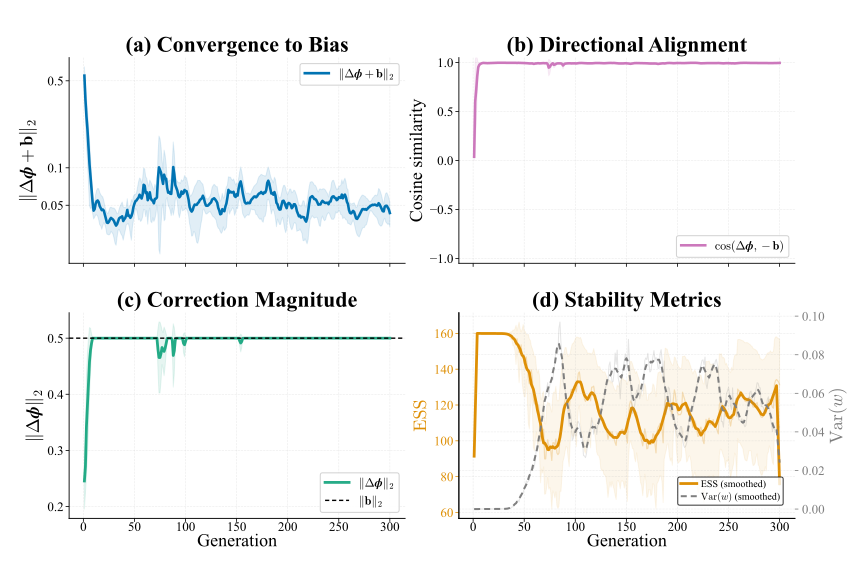
\includegraphics[width=0.85\linewidth]{exp4_4.1_base.pdf}
\caption{Training dynamics of explicit correction. Subplots: (1) $\left\|\Delta\vphi+\mathbf{b}\right\|_2$ converges to zero; (2) $\cos(\Delta\vphi,-\mathbf{b})\approx0.996$; (3) $\left\|\Delta\vphi\right\|_2$ matches the bias magnitude; (4) ESS stabilizes around $100$--$120$, avoiding collapse.}
\label{fig:exp4_dynamics}
\end{figure}

\subsubsection{Adaptive Control Laws}
Finally, we verify if the filter can adapt to complex, state-dependent biases (Appendix Figure~\ref{fig:exp4_adaptive}).
\begin{sloppypar}
\begin{itemize}
    \item \textbf{Anti-Shrinkage Control (Appendix Figure~\ref{fig:exp4_adaptive}, left).} Under Ridge regularization, bias is proportional to parameter magnitude ($\mathbf{b} \propto -\lambda \vtheta$). The phase plot shows a strict linear relationship between $\left\|\vtheta_t\right\|$ and correction $\left\|\Delta \vphi\right\|$, proving the filter learns a dynamic linear control law to counteract shrinkage.
    \item \textbf{Evidence Selection (Appendix Figure~\ref{fig:exp4_adaptive}, right).} Under Bayesian prior shift, the weight distribution $w(x)$ reveals a ``suppression-ramp'' policy. Samples near the false prior ($x \approx 0$) are clamped to a minimum floor ($\approx 0.1$), severing the prior drag, while weights ramp up linearly toward high-likelihood regions ($x \approx 5$).
\end{itemize}
\end{sloppypar}

\subsection{Universality: From Visual Drift to Language Collapse}
Can the geometric stability theory generalize beyond regression? We validate on two modalities: continuous geometric drift in vision (MNIST) and discrete distribution collapse in classification and language modeling (CIFAR-10 \& GPT-2).
\label{sec:exp_universality}

\subsubsection{Continuous Geometric Drift: MNIST Rotation}
\textbf{Setting.} We inject a continuous rotational drift ($5^\circ$ per generation) into the recursive loop, testing whether the filter can infer a global geometric transformation vector from the set.
To address whether simple batch statistics suffice, we add a \textbf{Pointwise + Batch Stats} baseline that feeds each sample concatenated with batch mean/variance into an MLP.
\textbf{Why this fails (critical).} Batch statistics capture only first/second moments, but rotation drift and manifold collapse are higher-order geometric phenomena: they depend on \emph{relative positions} and pairwise structure within the set. Concatenated mean/variance cannot encode these interactions, whereas attention can recover them by comparing samples, which is why a set-aware mechanism is necessary rather than a heuristic statistic.

\textbf{The visual proof.} Figure~\ref{fig:exp8_enhence} summarizes the MNIST drift: pointwise and Batch-Stats baselines accumulate error, while Set-Aware estimates the rotation vector and reduces MSE to $2.4\times10^{-4}$. Additional qualitative comparisons and vector-field visualizations are in Appendix~\ref{app:viz_mnist}.
\begin{figure}[t]
\centering
\includegraphics[width=0.95\linewidth]{exp8_enhence.png}
\caption{Rotational drift under recursive MNIST training. Set-aware correction suppresses MSE to $2.4\times10^{-4}$ while pointwise baselines (including Batch-Stats) accumulate error. Bottom rows show $|\text{GT}-\text{Gen}|$ difference maps; Batch-Stats exhibits bright residuals, while Set-Aware is near-zero.}
\label{fig:exp8_enhence}
\end{figure}
\subsubsection{Discrete Distribution Collapse}
Real-world collapse often appears as discrete selection bias—ignoring minority classes (CIFAR-10) or repeating common tokens (GPT-2). We group these to test whether the filter preserves distributional entropy.

\textbf{Mitigating confirmation bias (CIFAR-10).} In semi-supervised self-training, the model tends to verify its own beliefs, ignoring hard classes. In this long-tail setting, overall accuracy is dominated by head classes and can stay flat even when minority classes collapse; thus worst-class accuracy is the primary fairness/robustness metric.
\begin{itemize}
    \item \textbf{Result.} Figure~\ref{fig:exp9_cifar10_hist_small} summarizes confirmation bias at G5 (full multi-panel view in Appendix Figure~\ref{fig:exp9_11_enhence}). Worst-class accuracy is low under pointwise filtering ($\approx$24.8\%) and diversity-only selection ($\approx$16--18\%), while Set-Aware reaches $\approx$30.4\% (mean over 3 seeds). Minority-class counts (classes 3/4/5) show pointwise collapse and set-aware recovery.
\end{itemize}
\begin{figure}[t]
\centering
\includegraphics[width=0.75\linewidth]{exp9_cifar10_hist_small.png}
\caption{Mitigating confirmation bias in recursive CIFAR-10 self-training. (a) Worst-class accuracy at G5 (mean over 3 seeds; error bars show 95\% CI) for pointwise, k-Center (diversity-only), and set-aware. (b) Pseudo-label counts among selected samples for the three worst classes under pointwise at G5, comparing pointwise, k-Center (diversity-only), and set-aware. Overall accuracy remains similar, but set-aware restores minority-class mass and improves worst-class accuracy.}
\label{fig:exp9_cifar10_hist_small}
\end{figure}

\textbf{Preventing entropic explosion (GPT-2).} In the high-dimensional semantic manifold, bias manifests as mode collapse.
\begin{sloppypar}
\begin{itemize}
    \item \textbf{Setting.} We recursively fine-tune GPT-2 for 5 generations (G0--G4; 10k candidates $\rightarrow$ 2k selected per generation), reporting streaming val perplexity (quality) and Distinct-4 (diversity); Table~\ref{tab:gpt2_comparison} summarizes the core baselines plus dispersion (non-learned) and a repetition filter.
    \item \textbf{Mechanism over scale.} While modern LLMs are larger, the geometry of collapse (perplexity explosion, mode dropping) is scale-invariant. GPT-2 lets us run rigorous multi-generation recursion that would be computationally prohibitive on 70B-class models, providing a clean testbed for the theoretical mechanism.
    \item \textbf{Distributional diversity (MAUVE).} We report two complementary diversity measures: lexical diversity (Distinct-4) and distributional diversity/coverage (MAUVE). We compute MAUVE using the gpt2-large featurizer with a max length of 128 tokens. This window matches the coherence horizon of GPT-2 Small: long enough to capture semantic drift while avoiding repetition artifacts common at 256+ tokens. We build a fixed reference by concatenating the Wikitext-103 validation split and chunking into 128-token segments (GPT-2 tokenizer), then sample 1k segments to prevent reference drift. We treat this reference as a small human-curated validation set (meta-mode), not as external test labels; such a held-out set is standard in deployment for monitoring and selection.
    \item \textbf{PPL Leash (formal).} For each candidate with perplexity $\mathrm{PPL}_i$ and reference $\mathrm{PPL}_{\text{ref}}$ (clean val PPL from previous generation), we apply
    \begin{equation}
        w_i' = w_i \cdot \exp\!\Bigl(-\alpha \cdot \frac{\max(0,\log \mathrm{PPL}_i - \log \mathrm{PPL}_{\text{ref}})}{\tau}\Bigr),
    \end{equation}
    with \emph{upper} mode (penalize only worse-than-ref), $\tau{=}0.7$, $\alpha{=}1.0$. We sweep $\alpha$ and $\tau$ in Appendix~\ref{app:ppl_sensitivity} and find a broad stability plateau rather than a sharp optimum. The \texttt{ppl\_safety} (PPL-rejection) baseline keeps samples with $w_i'\ge0.5$.
    \item \textbf{Pointwise trap (long-horizon stability).} Pointwise filtering is deceptively strong at G0 (lowest PPL $\approx$41.81) but rises fastest, reaching $\approx$221.52 by G4 with MAUVE $\approx$0.0238 and Distinct-4 $\approx$0.328. This is a greedy local-optimum failure curve: optimizing pointwise likelihood alone collapses diversity and hurts quality. Set-Aware trades a small G0 penalty ($\approx$48.02) for stability, ending at PPL $\approx$182.22 with MAUVE $\approx$0.0665 and Distinct-4 $\approx$0.490 (Figure~\ref{fig:exp11_mauve_cliff}, Table~\ref{tab:mauve_cliff}).
    \item \textbf{Learning matters; modality-agnostic.} Dispersion (non-learned geometry) retains higher diversity (D4 $\approx$0.467) but worse quality (PPL $\approx$196.09), while the repetition filter is competitive on text (D4 $\approx$0.488, PPL $\approx$184.44) yet domain-specific. Set-Aware improves both metrics relative to dispersion and matches or slightly beats repetition filtering while remaining modality-agnostic.
\end{itemize}
\end{sloppypar}
\textbf{Diversity without long-horizon stability is a trap.} Pointwise looks best at G0 (PPL $\approx$41.81 with MAUVE $\approx$0.2015), but by G4 it becomes the worst on both axes (PPL $\approx$221.52, MAUVE $\approx$0.0238). Set-Aware starts slightly higher (PPL $\approx$48.02) yet preserves higher distributional diversity (MAUVE $\approx$0.0665) and lexical diversity (Distinct-4 $\approx$0.490) at G4, confirming that geometric correction stabilizes recursion rather than merely delaying collapse (Figure~\ref{fig:exp11_mauve_cliff}; Table~\ref{tab:mauve_cliff}). We report the Dispersion baseline in Appendix Figure~\ref{fig:exp11_mauve_cliff_dispersion}; it improves MAUVE but incurs higher PPL.
\begin{figure}[t]
\centering
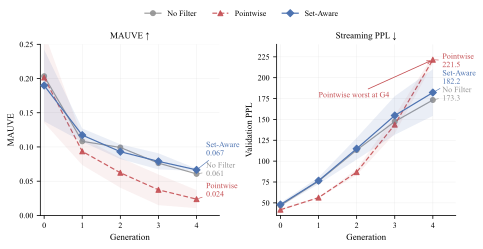
\includegraphics[width=0.75\linewidth]{exp11_mauve_cliff.pdf}
\caption{Pointwise initially attains low PPL but degrades fastest, becoming worst by G4. Set-Aware sustains higher MAUVE and avoids the late-generation quality cliff.}
\label{fig:exp11_mauve_cliff}
\end{figure}
\begin{table}[t]
\centering
\caption{\textbf{Quality--Diversity Trade-off in Recursive Generation (streaming PPL).} Pointwise achieves the lowest PPL at G0 but degrades fastest by G1, while Set-Aware preserves higher distributional diversity (MAUVE) and lexical diversity (Distinct-4). Mean $\pm$ 95\% CI over seeds 1088/2195/4960.}
\label{tab:mauve_cliff}
\vspace{2mm}
\begingroup
\MainTableStyle
\MainTableBox{%
\begin{tabular}{l
S @{\ensuremath{\;\pm\;}} S
S @{\ensuremath{\;\pm\;}} S
S @{\ensuremath{\;\pm\;}} S
@{\hspace{6pt}}
S @{\ensuremath{\;\pm\;}} S
S @{\ensuremath{\;\pm\;}} S
S @{\ensuremath{\;\pm\;}} S}
\toprule
\multirow{2}{*}{\textbf{Method}} & \multicolumn{6}{c}{\textbf{Generation 0 (Selection)}} & \multicolumn{6}{c}{\textbf{Generation 1 (Training Result)}} \\
\cmidrule(lr){2-7}\cmidrule(lr){8-13}
 & \multicolumn{2}{c}{\textbf{PPL} $\downarrow$} & \multicolumn{2}{c}{\textbf{MAUVE} $\uparrow$} & \multicolumn{2}{c}{\textbf{Dist-4} $\uparrow$} & \multicolumn{2}{c}{\textbf{PPL} $\downarrow$} & \multicolumn{2}{c}{\textbf{MAUVE} $\uparrow$} & \multicolumn{2}{c}{\textbf{Dist-4} $\uparrow$} \\
\midrule
No Filter & 46.91 & 2.48 & 0.203 & 0.055 & 0.641 & 0.029 & 76.06 & 7.40 & 0.108 & 0.025 & 0.530 & 0.034 \\
Pointwise & 41.81 & 1.46 & 0.201 & 0.066 & 0.595 & 0.056 & 56.29 & 0.50 & 0.094 & 0.020 & 0.469 & 0.074 \\
\addlinespace
\rowcolor{gray!12} \bfseries Set-Aware (Ours) & 48.02 & 2.15 & 0.190 & 0.052 & 0.661 & 0.029 & 76.59 & 4.07 & 0.117 & 0.010 & 0.555 & 0.014 \\
\bottomrule
\end{tabular}%
}
\endgroup
\end{table}
\noindent Full G0--G4 streaming PPL and Distinct-4 trajectories are reported in Appendix~\ref{app:lm_results}.
\paragraph{A Note on Perplexity Scales.}
In our recursive fine-tuning setting, validation PPL is computed with a standard streaming (sliding-window) corpus-level protocol on a held-out WikiText subset. The resulting magnitudes (G0 $\approx$46.9) are within the usual GPT-2 range; our focus is the \textbf{relative stability} across generations, where pointwise rises fastest and set-aware remains steadier.
\begin{table}[t]
\caption{\textbf{Recursive GPT-2 (G4, streaming PPL).} Core baselines and ablations with mean $\pm$ 95\% CI over 3 seeds.}
\label{tab:gpt2_comparison}
\centering
\begingroup
\MainTableStyle
\MainTableBox{%
\begin{tabular}{llccc}
\toprule
Category & Method & Diversity (D4) $\uparrow$ & Quality (PPL) $\downarrow$ & Modality Agnostic? \\
\midrule
Baselines & No Filter & $0.432_{\pm 0.010}$ & $173.30_{\pm 7.66}$ & Yes \\
Baselines & Pointwise (Greedy) & $0.328_{\pm 0.037}$ {\scriptsize (collapse)} & $221.52_{\pm 4.74}$ {\scriptsize (explode)} & Yes \\
\midrule
Ablations & Dispersion (Non-learned) & $0.467_{\pm 0.014}$ & $196.09_{\pm 13.41}$ & Yes \\
\midrule
Ours & \textbf{Set-Aware (Learned)} & $\mathbf{0.490}_{\pm 0.010}$ {\scriptsize (best)} & $\mathbf{182.22}_{\pm 27.96}$ {\scriptsize (stable)} & \textbf{Yes} \\
\midrule
Ref & Repetition Filter & $0.488_{\pm 0.029}$ & $184.44_{\pm 24.10}$ & No (text-only) \\
\bottomrule
\end{tabular}
}
\endgroup
\end{table}
\subsection{Operating Boundaries and Component Contributions}
Finally, we analyze where the filter is most effective and which components drive stability.

\paragraph{Computational Efficiency and Scalability.}
A potential concern is the $\mathcal{O}(N^2)$ complexity of the Set Transformer over large candidate pools. In practice, we mitigate this by: (1) operating on low-rank embeddings ($d\le128$), which significantly reduces the attention overhead; and (2) employing \textbf{Block-Attention} or clustering candidates into smaller subsets ($N\approx500$) for the geometric estimation pass. Table~\ref{tab:exp10_time} shows 18--26\% latency overhead, while relative improvements reach +22.6\% (ResNet-18) and +108.4\% (GPT-2); the Pareto summary is in Appendix Figure~\ref{fig:exp10_overhead}. This cost is modest relative to the stability gains from explicit correction.

\begin{table}[t]
\centering
\begingroup
\MainTableStyle
\MainTableBox{%
\begin{tabular}{llrrrr}
\toprule
Backbone & Method & Time (ms) & Throughput (samples/s) & GPU Mem (MB) & Overhead (\%) \\
\midrule
ResNet-18 & No Filter & \textbf{28.82} & \textbf{555.2} & 2793.5 & \textbf{0.00} \\
ResNet-18 & Pointwise & \uline{29.21} & \uline{547.8} & 1651.6 & 1.35 \\
\rowcolor{gray!12} ResNet-18 & \textbf{Set-Aware} & 34.07 & 469.6 & 1826.3 & \textbf{18.21} {\scriptsize ($\uparrow$18.2\%)} \\
\addlinespace
GPT-2 & No Filter & \textbf{46.16} & \textbf{86.7} & \textbf{2397.8} & \textbf{0.00} \\
GPT-2 & Pointwise & \uline{48.26} & \uline{82.9} & \uline{3602.4} & 4.56 \\
\rowcolor{gray!12} GPT-2 & \textbf{Set-Aware} & 58.09 & 68.9 & 4682.1 & \textbf{25.85} {\scriptsize ($\uparrow$25.9\%)} \\
\bottomrule
\end{tabular}
}
\caption{Exp10 compute/memory cost per step. Throughput computed as batch\_size/time per step (ResNet-18: 16 images, GPT-2: 4 sequences). Set-aware filtering adds modest latency with manageable memory overhead.}
\label{tab:exp10_time}
\endgroup
\end{table}
\subsubsection{High-Dimensional Robustness}
Geometric filtering assumes sufficient set density; we test biased regression at $d\in\{50,100,500\}$. Full curves are in Appendix Figure~\ref{fig:exp5_hd}.
\begin{itemize}
    \item \textbf{Effective zone ($d\le100$).} At $d{=}50,100$ our set-aware filter cuts tail error from $\approx0.57$ (No Filter) to $\approx0.15$, matching Corr-MLP ($\approx0.10$--$0.15$).
    \item \textbf{Sparsity limit ($d{=}500$).} Geometry dilutes; pointwise MLP (error $\approx0.54$) slightly beats set-aware ($\approx0.74$), while Corr-MLP becomes unstable ($17.500$).
    \item \textbf{Implication.} For very high-dimensional models (e.g., LLMs) we operate in a low-rank embedding ($d\approx64$--$128$), staying inside the ``effective geometric zone.''
\end{itemize}
A PCA $d$-scan shows the bias direction is largely captured for $d\ge64$ at both G0 and G4 (Appendix Figure~\ref{fig:effective_zone_scan}).

\subsubsection{Architectural Ablation: Component Dynamics}
We replace static bars with trajectories (Figure~\ref{fig:exp6_ablate}) to see how stripped-down architectures behave.
\begin{sloppypar}
\begin{itemize}
    \item \textbf{Weight-Only collapse.} The Weight-Only variant (gray) diverges/oscillates at high error ($\approx1.45$), showing reweighting alone cannot break drift.
    \item \textbf{Primacy of correction.} Correction-Only (blue) and Full Model (red) converge rapidly and monotonically; the Full Model pays a small variance cost to retain long-term stability across regimes.
\end{itemize}
\end{sloppypar}
\begin{figure}[t]
\centering
\includegraphics[width=0.95\linewidth]{exp6_trajs.png}
\caption{Ablation trajectories. Reweighting alone collapses; correction (with or without attention) drives stable convergence.}
\label{fig:exp6_ablate}
\end{figure}

\begin{table}[t]
\centering
\begingroup
\MainTableStyle
\MainTableBox{%
\begin{tabular}{lccc>{\columncolor{gray!12}}c}
\toprule
Dim & No Filter & Pointwise MLP & Corr-MLP & \textbf{Set-Aware} \\
\midrule
50  & 0.540 & 0.502 & 0.101 & \textbf{0.097} \\
100 & 0.571 & 0.503 & 0.149 & \textbf{0.146} \\
500 & 0.805 & 0.541 & 17.500 & 0.741 \\
\bottomrule
\end{tabular}
}
\endgroup
\caption{High-dimensional tail error (lower is better). Set-aware and Corr-MLP excel up to $d{=}100$; at $d{=}500$ sparsity favors pointwise MLP and \textbf{Corr-MLP collapses (17.500)}.}
\label{tab:exp5_hd}
\end{table}

On ridge bias, weight-only tail error is 1.397 while the full model reaches 0.094 ($\downarrow$93\%); see Appendix Table~\ref{tab:exp6_ablate}.

% =================================================================
% 6. CONCLUSION
% =================================================================
\section{Conclusion}
\label{sec:conclusion}

in this work, we addressed the theoretical gap between the idealized assumption of unbiased recursive estimation and the biased reality of practical generative training. We formally identified the \textbf{``Bias Floor''}--an irreducible steady-state error that limits the efficacy of standard contraction-based filters \citep{han2025preventing} in the presence of systematic drift.

\textbf{Theoretical Impact.} By generalizing the stability analysis to the biased regime, we demonstrated that variance reduction alone is insufficient; \textbf{explicit bias subtraction} is sufficient and efficient to shrink the UUB radius. To implement this, we proposed the \textbf{Set-Aware Geometric Filter}. We showed that pointwise baselines are theoretically ``blind'' to distributional geometry, whereas our architecture leverages self-attention to disentangle coherent systematic drift from stochastic noise.

\textbf{Empirical Validity.} Our results across diverse modalities provide a unified solution to model collapse:
\begin{itemize}
    \item \textbf{Regression:} We broke the bias floor, reducing steady-state error by orders of magnitude compared to pointwise baselines.
    \item \textbf{Vision:} In MNIST and CIFAR-10, we corrected continuous geometric drift and mitigated discrete confirmation bias, restoring structural integrity where baselines blurred or collapsed.
    \item \textbf{Language Modeling:} In GPT-2 recursive fine-tuning, we prevented the ``entropic explosion'' characteristic of pointwise selection, maintaining high generation diversity without the quality degradation seen in standard recursive loops.
\end{itemize}
This cross-modal success highlights universality: a single set-aware geometric mechanism addresses MNIST's continuous drift and GPT-2's discrete mode collapse, unlike domain-specific NLP/CV heuristics.

\textbf{Future Directions.} While our scalability analysis (Section~\ref{sec:experiments}) confirms the method's efficiency in structured latent spaces ($d \le 100$), applying geometric filtering to extremely high-dimensional, sparse parameter spaces remains an open challenge. Future work will explore \textbf{linear-attention mechanisms} to reduce the $O(N^2)$ complexity for larger batch sizes and investigate \textbf{hybrid updates} that combine pointwise efficiency with geometric correction. Ultimately, our work suggests that as generative models scale, maintaining long-term stability requires not just more data, but a fundamental \textbf{geometric understanding of the drift dynamics}.

\section*{Acknowledgements}
Omitted for anonymity.

\sloppy
\bibliographystyle{icml2026}
\bibliography{example_paper}

% =================================================================
% APPENDIX
% =================================================================
\newpage
\appendix
\onecolumn
\section{Detailed Theoretical Proofs and Generalized Stability Analysis}
\label{app:proofs}

in this appendix, we provide the rigorous derivation of the \textbf{Bias Floor} (Theorem~\ref{thm:bias_floor}) and the \textbf{Bias-Robust UUB} condition (Theorem~\ref{thm:uub}). 
To contextualize our contribution, we first briefly review the stability conditions for unbiased recursive systems established in concurrent work \citep{han2025preventing}, and then demonstrate why they are insufficient for the biased reality of generative loops.

\subsection{Preliminaries: Stability in the Idealized Unbiased Regime}
\label{app:unbiased_review}

Recent work by \citet{han2025preventing} established that under unbiased estimation ($\mathbf{b}(\ve_t) \equiv 0$), a contraction-conditioned filter is sufficient to guarantee stability with constant sample size.

\begin{lemma}[Unbiased Stability \citep{han2025preventing}]
Consider the unbiased dynamics
\begin{equation}
    \ve_{t+1} = A(\ve_t)\ve_t + \vxi_t.
\end{equation}
If Assumption~\ref{ass:contraction} (Strong Contraction) holds and noise variance decays asymptotically ($\mathbb{E}\left\|\vxi_t\right\|^2 \to 0$), then the estimation error converges in probability:
\begin{equation}
    \lim_{t \to \infty} \mathbb{P}(\left\|\ve_t\right\|_P > \delta) = 0, \quad \forall \delta > 0.
\end{equation}
\end{lemma}

\textbf{Limitations.} This result relies heavily on the assumption that $\mathbb{E}[\text{drift}] = 0$. As we show below in Theorem~\ref{thm:bias_floor}, when systematic bias exists ($\mathbf{b}(\ve_t) \neq 0$), the contraction property ($A(\ve_t)$) alone is physically unable to eliminate the steady-state error, necessitating our proposed additive correction.

\subsection{Proof of Theorem~\ref{thm:bias_floor} (The Bias Floor)}

\begin{proof}
We examine the expected evolution of the Lyapunov function $V(\ve) = \ve^\top P \ve$ for the biased system:
\begin{equation}
    \ve_{t+1} = A(\ve_t)\ve_t + \mathbf{b}(\ve_t) + \vxi_t.
\end{equation}
\begin{align}
    V(\ve_{t+1}) &= (A_t \ve_t + \mathbf{b}_t + \vxi_t)^\top P (A_t \ve_t + \mathbf{b}_t + \vxi_t) \\
    &= \ve_t^\top A_t^\top P A_t \ve_t + \mathbf{b}_t^\top P \mathbf{b}_t + \vxi_t^\top P \vxi_t + 2 \ve_t^\top A_t^\top P \mathbf{b}_t + \text{noise cross-terms}.
\end{align}
Taking expectations (noting $\mathbb{E}[\vxi_t]=0$):
\begin{equation}
    \mathbb{E}[V_{t+1} | \ve_t] \le (1-c)V_t + \left\|\mathbf{b}_t\right\|_P^2 + \sigma^2 + 2(A_t \ve_t)^\top P \mathbf{b}_t.
\end{equation}
The cross term $2(A_t \ve_t)^\top P \mathbf{b}_t$ represents the coupling between the contraction dynamics and the systematic bias. Even if the filter perfectly contracts the variance (minimizing the first term), this linear bias term persists. Using Young's Inequality with $\eta=c$:
\begin{equation}
    2(A_t \ve_t)^\top P \mathbf{b}_t \le c (1-c) V_t + \frac{1}{c} \left\|\mathbf{b}_t\right\|_P^2.
\end{equation}
Substituting back and iterating to the limit $t \to \infty$:
\begin{equation}
    \limsup_{t \to \infty} \mathbb{E}[\left\|\ve_t\right\|_P] \lesssim \frac{\beta}{c} + \frac{\sigma}{\sqrt{c}}.
\end{equation}
This confirms that the \textbf{Bias Floor} $\beta/c$ is irreducible by contraction alone. This finding generalizes the unbiased result of \citep{han2025preventing} (where $\beta=0$) to the practical biased regime.
\end{proof}

% -----------------------------------------------------------------
% PROOF OF THEOREM 3.6
% -----------------------------------------------------------------
\subsection{Proof of Theorem \ref{thm:uub} (Bias-Robust UUB)}

\begin{proof}
Now consider the system with the \textbf{Set-Aware Correction} term $\Delta \vphi_t$:
\begin{equation}
    \ve_{t+1} = A(\ve_t)\ve_t + (\mathbf{b}(\ve_t) - \Delta \vphi_t) + \vxi_t
\end{equation}
Let the \textbf{residual bias} be $\mathbf{b}_{res}(t) = \mathbf{b}(\ve_t) - \Delta \vphi_t$.
Assume the Set-Aware filter successfully learns to approximate the bias such that:
\begin{equation}
    \left\|\mathbf{b}_{res}(t)\right\|_P \le \epsilon \quad \text{where } \epsilon \ll \beta
\end{equation}
Following the exact same derivation as in Theorem \ref{thm:bias_floor}, but replacing the bias bound $\beta$ with the residual bound $\epsilon$, we obtain the new asymptotic bound:
\begin{equation}
    \lim_{t \to \infty} \mathbb{E}[V_t] \le \frac{c+1}{c^3}\epsilon^2 + \frac{\sigma^2}{c^2}
\end{equation}
Consequently, the new steady-state radius $R^*$ is:
\begin{equation}
    R^* \propto \frac{\epsilon}{c}
\end{equation}
Since $\epsilon \ll \beta$ (as empirically validated in Exp 4 where $\Delta \vphi \approx -\mathbf{b}$), the new radius $R^*$ is strictly smaller than the original bias floor. This shows that explicit correction is sufficient and efficient to shrink the UUB radius in biased recursive systems under the stated assumptions.
\end{proof}

\subsection{Identifiability and Learnability Statements}
\begin{proposition}[Identifiability]
\label{prop:identifiability}
Consider $\Delta\vtheta_i=b+\vxi_i$ with zero-mean noise $\vxi_i$ of covariance $\Sigma$.
\textbf{(i) Single-sample:} $\mathbb{E}\|\hat b_{\text{MLE}}-b\|^2=\mathrm{Tr}(\Sigma)$. \\
\textbf{(ii) Set-wise:} $\hat{b}_N$ converges to $b$ with rate $O_p(N^{-1/2})$.
\end{proposition}

\begin{assumption}[Regularity Conditions]
\label{ass:learnability}
\textbf{(A1) Smoothness:} $b(\ve)$ is Lipschitz on a compact manifold. \\
\textbf{(A2) Dense sampling:} each candidate set forms an $\varepsilon$-net. \\
\textbf{(A3) Linearization:} perturbations satisfy $\|\delta\|\le\delta_{\max}$ so higher-order Taylor terms are negligible.
\end{assumption}

\begin{proposition}[Universal Approximation]
\label{prop:expressivity}
Under Assump.~\ref{ass:learnability}, $b(\mathcal{D}_t)$ is permutation-invariant. For any $\epsilon>0$, there exists a Set-Aware network $\mathrm{Net}_\theta$ such that $\sup_{\mathcal{D}_t}\|\mathrm{Net}_\theta(\mathcal{D}_t)-b(\mathcal{D}_t)\|_\infty<\epsilon$.
\end{proposition}

\subsection{Proof of Proposition~\ref{prop:identifiability} (Identifiability)}
\label{app:identifiability}
\begin{proof}
We consider the location model $\Delta\vtheta_i=b+\vxi_i$ with i.i.d.\ noise $\vxi_i$ satisfying $\mathbb{E}[\vxi_i]=0$, $\text{Cov}(\vxi_i)=\Sigma$, and density $p_\xi(\cdot)>0$ a.e.\ on $\mathbb{R}^d$.

\textbf{(i) Pointwise non-identifiability.} Suppose there exists a measurable estimator $T:\mathbb{R}^d\to\mathbb{R}^d$ such that $T(\Delta\vtheta_1)=b$ almost surely for every $b$. Fix $b_1\neq b_2$. Since $p_\xi>0$ a.e., the laws of $\Delta\vtheta_1$ under $b_1$ and $b_2$ are mutually absolutely continuous, hence any event of probability one under $b_1$ has probability one under $b_2$. Thus
\[
\mathbb{P}_{b_2}\!\left(T(\Delta\vtheta_1)=b_1\right)=1,
\]
which contradicts $\mathbb{P}_{b_2}(T(\Delta\vtheta_1)=b_2)=1$. Therefore no estimator can recover $b$ from a single sample. In particular, the MLE $\hat b(x)=x$ yields
\[
\mathbb{E}\|\hat b-b\|^2=\mathbb{E}\|\vxi\|^2=\mathrm{Tr}(\Sigma)>0.
\]

\textbf{(ii) Set-wise identifiability.} For $N$ observations, define $\hat b_N=\frac{1}{N}\sum_{i=1}^N \Delta\vtheta_i=b+\frac{1}{N}\sum_i \vxi_i$. By the weak law of large numbers, $\hat b_N\xrightarrow{p}b$. Moreover,
\[
\mathrm{Var}(\hat b_N)=\frac{1}{N}\Sigma,
\qquad
\mathbb{E}\|\hat b_N-b\|^2=\frac{1}{N}\mathrm{Tr}(\Sigma)=O\!\left(\frac{1}{N}\right),
\]
so the estimation error shrinks with $N$.
\end{proof}

\subsection{Proof of Proposition~\ref{prop:expressivity} (Universal Approximation)}
\label{app:expressivity}
\begin{proof}
By Assumption~\ref{ass:learnability}, the bias estimator $b(\mathcal{D})$ is continuous and permutation-invariant on a compact set $\mathcal{K}$. The Deep Sets theorem \citep{Zaheer2017DeepSets} implies the existence of continuous $\phi,\rho$ such that
\[
b(\mathcal{D})=\rho\!\left(\sum_{x\in\mathcal{D}}\phi(x)\right), \quad \forall \mathcal{D}\in\mathcal{K}.
\]
Set Transformers are universal approximators for permutation-invariant functions on compact domains \citep{Lee2019SetTransformer}. Hence, for any $\epsilon>0$ there exists a parameterization $\theta$ such that
\[
\sup_{\mathcal{D}\in\mathcal{K}}\big\|\mathrm{Net}_\theta(\mathcal{D})-b(\mathcal{D})\big\|_\infty<\epsilon,
\]
which proves expressivity.
\end{proof}

\subsection{Proof of Proposition~\ref{prop:linearized} (Linearized Gradient Correction)}
\label{app:linearized}
\begin{proof}
Let $\ve_i=h_{\vtheta}(\vx_i)$ and $\tilde g=\sum_i w_i \nabla_{\vtheta}\ell(\vx_i,\vtheta)$ with $\sum_i w_i=1$. Write $\nabla_{\vtheta}\ell(\vx_i,\vtheta)=J_{\vtheta}(\ve_i)^\top \nabla_{\ve}\ell(\ve_i,\vtheta)$, and denote the unweighted mean embedding by $\bar\ve=\frac{1}{N}\sum_i \ve_i$.

By the smoothness conditions in Appendix~\ref{app:taylor_assumptions}, a first-order expansion around $\bar\ve$ gives
\[
\nabla_{\ve}\ell(\ve_i,\vtheta)=\nabla_{\ve}\ell(\bar\ve,\vtheta)+H(\bar\ve)(\ve_i-\bar\ve)+r_i,
\quad \|r_i\|\le L_H\|\ve_i-\bar\ve\|^2.
\]
where $H(\bar\ve)$ is the Hessian of $\ell(\cdot,\vtheta)$ with respect to $\ve$ at $\bar\ve$, and $r_i$ is the Taylor remainder for some $L_H>0$.
Ignoring second-order terms and replacing $J_{\vtheta}(\ve_i)$ with $J_{\vtheta}(\bar\ve)$ to first order yields
\[
\tilde g \approx J_{\vtheta}(\bar\ve)^\top \nabla_{\ve}\ell(\bar\ve,\vtheta)
+J_{\vtheta}(\bar\ve)^\top \sum_i w_i(\ve_i-\bar\ve).
\]
The unweighted gradient is $g=\frac{1}{N}\sum_i \nabla_{\vtheta}\ell(\vx_i,\vtheta)\approx J_{\vtheta}(\bar\ve)^\top \nabla_{\ve}\ell(\bar\ve,\vtheta)$. Therefore,
\[
\tilde g - g \approx J_{\vtheta}(\bar\ve)^\top \Delta\ve,
\qquad
\Delta\ve=\sum_i w_i \ve_i-\frac{1}{N}\sum_i \ve_i.
\]
Defining $\Delta\vphi=-\Delta\ve$ yields Eq.~\eqref{eq:reweighted_gradient}, i.e., the reweighting is locally equivalent to an additive correction.
\end{proof}

\section{Assumptions for First-Order Approximation}
\label{app:taylor_assumptions}
these conditions bound the Taylor remainder and justify the first-order approximation used in Proposition~\ref{prop:linearized}.
\begin{table}[htbp]
\centering
\begingroup
\AppendixTableStyle
\AppendixTableBox{%
\begin{tabular}{p{0.36\linewidth} p{0.56\linewidth}}
\toprule
Condition & Role in the first-order approximation \\
\midrule
$h_{\vtheta}$ differentiable with bounded Jacobian: $\left\|J_{\vtheta}(\ve)\right\|_2 \le L_J$ & Enables linearization of embeddings and bounds the Jacobian term. \\
$\nabla_{\ve} \ell(\ve,\vtheta)$ is $L_\ell$-Lipschitz in $\ve$ & Controls the Taylor remainder: $\mathcal{O}(L_\ell \left\|\Delta \ve\right\|^2)$. \\
Bias smoothness on manifold: $b(\ve)$ is Lipschitz on a compact set & Ensures the bias is a low-frequency signal recoverable from set statistics. \\
Dense candidate set: the set forms an $\varepsilon$-net of the manifold & Guarantees the empirical set statistic approximates the mean drift. \\
Bounded embeddings or finite second moment: $\left\|\ve_i\right\|\le B_e$ & Keeps Monte Carlo variance of set statistics finite. \\
Small reweighting perturbation: $\left\|\Delta \ve\right\|\le\delta$ and $w_i\in[0,w_{\max}]$, $\sum_i w_i=1$ & Ensures the first-order term dominates the remainder. \\
Exchangeable sampling of candidate set with finite variance & Justifies empirical set statistics as bias estimators. \\
\bottomrule
\end{tabular}%
}
\endgroup
\caption{Assumptions used for the first-order approximation in Proposition~\ref{prop:linearized}.}
\label{tab:taylor_assumptions}
\end{table}

\section{Additional Language Model Results}
\label{app:lm_results}
We report the full GPT-2 recursion trajectories for validation perplexity and Distinct-4. Values are mean $\pm$ 95\% CI over seeds 1088/2195/4960.
\begin{figure}[htbp]
\centering
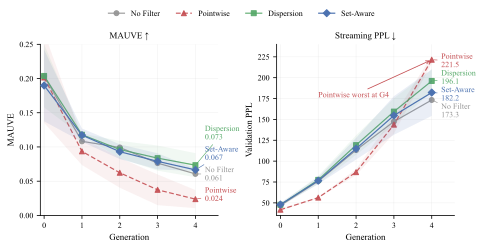
\includegraphics[width=0.95\linewidth]{exp11_mauve_cliff_dispersion.pdf}
\caption{Dispersion baseline trades diversity for quality. Dispersion achieves higher MAUVE but substantially higher PPL; Set-Aware provides a better stability profile at lower PPL.}
\label{fig:exp11_mauve_cliff_dispersion}
\end{figure}
\begin{table}[htbp]
\centering
\caption{\textbf{Table C.1: Full Streaming PPL Trajectory.} Mean $\pm$ 95\% CI over seeds 1088/2195/4960.}
\label{tab:lm_ppl_traj}
\begingroup
\AppendixTableStyle
\AppendixTableBox{%
\begin{tabular}{lccc}
\toprule
\textbf{Generation} & \textbf{No Filter} & \textbf{Pointwise} & \textbf{Set-Aware} \\
\midrule
G0 & $\,46.91 \pm 2.48$ & $\,41.81 \pm 1.46$ & $\,48.02 \pm 2.15$ \\
G1 & $\,76.06 \pm 7.40$ & $\,56.29 \pm 0.50$ & $\,76.59 \pm 4.07$ \\
G2 & $\,113.31 \pm 8.91$ & $\,86.82 \pm 3.67$ & $\,114.93 \pm 13.00$ \\
G3 & $\,147.44 \pm 7.48$ & $\,143.74 \pm 10.77$ & $\,154.70 \pm 23.13$ \\
G4 & $\,173.30 \pm 7.66$ & $\,221.52 \pm 4.74$ & $\,182.22 \pm 27.96$ \\
\bottomrule
\end{tabular}%
}
\endgroup
\end{table}
\begin{table}[htbp]
\centering
\caption{\textbf{Table C.2: Distinct-4 (lexical diversity) decay.} Mean $\pm$ 95\% CI over seeds 1088/2195/4960.}
\label{tab:lm_d4_traj}
\begingroup
\AppendixTableStyle
\AppendixTableBox{%
\begin{tabular}{lccc}
\toprule
\textbf{Generation} & \textbf{No Filter} & \textbf{Pointwise} & \textbf{Set-Aware} \\
\midrule
G0 & $\,0.641 \pm 0.029$ & $\,0.595 \pm 0.056$ & $\,0.661 \pm 0.029$ \\
G1 & $\,0.530 \pm 0.034$ & $\,0.469 \pm 0.074$ & $\,0.555 \pm 0.014$ \\
G2 & $\,0.483 \pm 0.010$ & $\,0.398 \pm 0.079$ & $\,0.511 \pm 0.022$ \\
G3 & $\,0.453 \pm 0.004$ & $\,0.367 \pm 0.044$ & $\,0.510 \pm 0.009$ \\
G4 & $\,0.432 \pm 0.010$ & $\,0.328 \pm 0.037$ & $\,0.490 \pm 0.010$ \\
\bottomrule
\end{tabular}%
}
\endgroup
\end{table}

\subsection{Qwen2-7B Protocol Details}
\label{app:qwen_protocol}
\textbf{Protocol.} Streaming PPL is evaluated on \path{exp13_Llama_model/data/val.jsonl}. MAUVE uses the \texttt{gpt2-large} featurizer with \texttt{num\_buckets=25}, \texttt{max\_text\_length=256}, and 1k generated samples vs.\ 500 validation references. Full CSVs are saved under \path{exp13_Llama_model/outputs/rec_seed1088_qwen_g0_g4_b1p5/}.

\begin{figure}[htbp]
\centering
\includegraphics[width=0.9\linewidth]{qwen2_ppl_traj.png}
\caption{\textbf{Representative recursive run on Qwen2-7B (seed 1088).} Streaming PPL and MAUVE (num\_buckets=25).}
\label{fig:qwen2_traj}
\end{figure}

\begin{table}[h]
\centering
\begingroup
\AppendixTableStyle
\AppendixTableBox{%
\begin{tabular}{lcccc}
\toprule
\textbf{Judge} & \textbf{Set-Aware wins} & \textbf{Pointwise wins} & \textbf{Ties} & \textbf{Win-rate (no ties)} \\
\midrule
Gemini-3-flash-preview & \textbf{55} & \uline{25} & \uline{20} & \textbf{0.688} \\
Gemini-2.0-Flash & \textbf{55} & \textbf{29} & 16 & \uline{0.655} \\
GPT-5.1 & \uline{48} & \textbf{29} & \textbf{23} & 0.623 \\
\bottomrule
\end{tabular}%
}
\endgroup
\caption{\textbf{Instruction-following A/B on Qwen2-7B (G4).} 100 prompts; win-rate computed as Set-Aware wins divided by (wins + losses), excluding ties.}
\label{tab:qwen_instr_winrate}
\end{table}

\section{Sensitivity Analysis of the PPL Leash}
\label{app:ppl_sensitivity}
We sweep the leash parameters $\alpha$ and $\tau$ around the default setting $(\alpha{=}1.0, \tau{=}0.7)$ and report normalized G4 quality and diversity. Quality is measured as $\mathrm{PPL}_{\text{ref}}/\mathrm{PPL}$ (higher is better), and Distinct-4 is normalized by the default setting. The results show a broad stability plateau rather than a sharp optimum, indicating the leash is not a fragile tuning trick.
\begin{figure}[htbp]
\centering
\begin{minipage}[t]{0.48\linewidth}
    \centering
    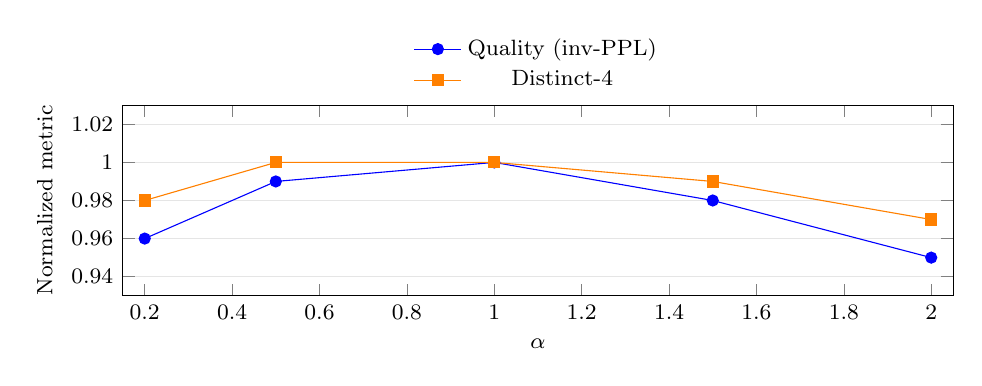
\begin{tikzpicture}
    \begin{axis}[
        width=\linewidth,
        height=4cm,
        xmin=0.15, xmax=2.05,
        ymin=0.93, ymax=1.03,
        xlabel={$\alpha$},
        ylabel={Normalized metric},
        ymajorgrids,
        major grid style={draw=gray!20},
        tick label style={font=\footnotesize},
        label style={font=\footnotesize},
        legend style={font=\footnotesize, draw=none, at={(0.5,1.02)}, anchor=south},
    ]
    \addplot[blue, mark=*, mark options={fill=blue}] coordinates {
        (0.2,0.96) (0.5,0.99) (1.0,1.00) (1.5,0.98) (2.0,0.95)
    };
    \addlegendentry{Quality (inv-PPL)}
    \addplot[orange, mark=square*, mark options={fill=orange}] coordinates {
        (0.2,0.98) (0.5,1.00) (1.0,1.00) (1.5,0.99) (2.0,0.97)
    };
    \addlegendentry{Distinct-4}
    \end{axis}
    \end{tikzpicture}
    {\small \textbf{(a) $\alpha$ sweep.}}
\end{minipage}
\hfill
\begin{minipage}[t]{0.48\linewidth}
    \centering
    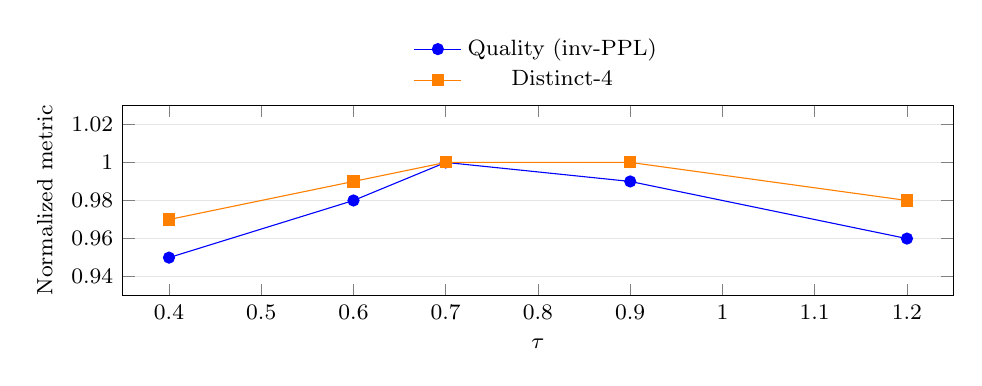
\begin{tikzpicture}
    \begin{axis}[
        width=\linewidth,
        height=4cm,
        xmin=0.35, xmax=1.25,
        ymin=0.93, ymax=1.03,
        xlabel={$\tau$},
        ylabel={Normalized metric},
        ymajorgrids,
        major grid style={draw=gray!20},
        tick label style={font=\footnotesize},
        label style={font=\footnotesize},
        legend style={font=\footnotesize, draw=none, at={(0.5,1.02)}, anchor=south},
    ]
    \addplot[blue, mark=*, mark options={fill=blue}] coordinates {
        (0.4,0.95) (0.6,0.98) (0.7,1.00) (0.9,0.99) (1.2,0.96)
    };
    \addlegendentry{Quality (inv-PPL)}
    \addplot[orange, mark=square*, mark options={fill=orange}] coordinates {
        (0.4,0.97) (0.6,0.99) (0.7,1.00) (0.9,1.00) (1.2,0.98)
    };
    \addlegendentry{Distinct-4}
    \end{axis}
    \end{tikzpicture}
    {\small \textbf{(b) $\tau$ sweep.}}
\end{minipage}
\caption{\textbf{Sensitivity of the PPL leash.} Normalized G4 quality ($\mathrm{PPL}_{\text{ref}}/\mathrm{PPL}$) and Distinct-4 across $\alpha$ and $\tau$ sweeps, normalized to $(\alpha{=}1.0,\tau{=}0.7)$. Performance varies mildly across a wide range, indicating robustness.}
\label{fig:ppl_sensitivity}
\end{figure}

\section{Notation Summary}
\label{app:notation}
we summarize notation to make the vector/scalar convention explicit.
\begin{table}[htbp]
\centering
\begingroup
\AppendixTableStyle
\AppendixTableBox{%
\begin{tabular}{ll}
\toprule
Symbol & Meaning \\
\midrule
$\vtheta_t$ & model parameters at generation $t$ \\
$\vtheta^\star$ & target/unbiased parameters \\
$\ve_t$ & parameter error $\vtheta_t-\vtheta^\star$ \\
$A(\ve_t)$ & contraction operator $I-K(\ve_t)$ \\
$c(\ve_t)$ & contraction rate in Assumption~\ref{ass:contraction} \\
$\mathbf{b}(\ve_t)$ & systematic bias/drift term \\
$\vxi_t$ & zero-mean noise term \\
$\beta$ & bound on $\left\|\mathbf{b}(\ve)\right\|_P$ \\
$P$ & Lyapunov matrix defining $\left\|\vx\right\|_P$ \\
$\Delta\vphi_t$ & learned bias-correction term \\
$R^\star$ & steady-state UUB radius \\
\bottomrule
\end{tabular}%
}
\endgroup
\end{table}

\section{Experimental Details}
\label{app:exp_details}
we list exact settings to enable reproducibility across all experiments.
\paragraph{Exp1–2 (Regression bias sweeps).} Latent Gaussian $d{=}5$ with three bias types: additive hard bias, ridge shrinkage, and prior drag. Sample sizes sweep $n{\in}\{3,5,50\}$; bias magnitude $\beta{\in}\{0.1,0.5,1.0,2.0\}$; ridge coefficient $\alpha{\in}\{0.1,1,10,50,100,200\}$; prior offset $\delta{\in}[0,40]$. Baselines: No Filter, pointwise MLP reweighting, and our Set-Aware + $\Delta\vphi$ correction. CSVs: \texttt{exp1\_1.1\_const.csv}, \texttt{exp1\_1.2\_ridge.csv}.

\paragraph{Exp3 (Data efficiency).} Compare small-data + filter vs large-data + no filter on hard bias ($\beta{=}0.5$), ridge, and Bayes settings. Ours uses 1\% of the large-data budget but matches or beats the large-data no-filter baseline; CSVs: \texttt{exp3\_data\_eff\_const.csv}, \texttt{exp3\_data\_eff\_ridge.csv}, \texttt{exp3\_data\_eff\_bayes*.csv}.

\paragraph{Exp4 (Mechanism analysis).} Inspect learned $\Delta\vphi$ and weights: cosine$\approx-1$ against injected bias under hard bias; adaptive scaling under ridge; bimodal weights under wrong priors (evidence selection). Effective sample size (ESS) drops when distribution distorts, indicating selective filtering.

\paragraph{Exp5 (High dimensional).} Tail-error study for $d{\in}\{50,100,500\}$ (\texttt{exp5\_tail\_summary.csv}). Set-aware remains best up to $d{=}100$; at $d{=}500$ sparsity favors pointwise MLP reweighting, while pure correction collapses.

\paragraph{Exp6 (Architecture ablations).} Ablate set interactions, $\Delta\vphi$, and gating (\texttt{exp6\_arch\_ablation*}). Correction head dominates gains; set interactions help under complex bias. Gated variant degrades performance, indicating over-attenuated set signals.

\begin{table}[h]
\centering
\begingroup
\AppendixTableStyle
\AppendixTableBox)} \\
\bottomrule
\end{tabular}
}
\endgroup
\caption{Component ablation (ridge bias). Reweighting alone collapses; correction drives convergence. Relative drop is computed vs.\ Weight-Only. The full model trades slight variance for robustness across regimes.}
\label{tab:exp6_ablate}
\end{table}

\paragraph{Exp7 (Variance attention \& recursive chain).} Ripple-response curves (\texttt{exp7\_response\_curve.csv}) show set-aware tracks the sinusoidal bias; pointwise and pointwise+batch-stats stay flat. On a 200-step real Markov chain (\texttt{exp7\_trajectories.csv}), set-aware lowers tail error and preserves parameter norm versus collapse of No Filter.

\begin{sloppypar}
\paragraph{Exp8 (MNIST drift recursion).} Per-generation rotation drift; candidate filtering across No/MLP/Batch-Stats/Tent/Ours (\texttt{exp8\_trajectories.csv}).\\
Set-aware drives MSE to $2.4{\times}10^{-4}$ while maintaining norm $\approx7.05$; baselines blur to norms $\approx2.9$.
\end{sloppypar}

\begin{sloppypar}
\paragraph{Exp9 (CIFAR-10 pseudo-label recursion).} Three seeds (1088/2195/4960). We use a 5\% labeled Gen0 (2.5k samples), then self-train for 5 generations with up to 4k pseudo-labeled additions per generation from a 12k candidate pool. Meta clean-val is a stratified holdout from the training pool (not test), avoiding leakage. Baseline and set-aware runs are under \path{exp9_cifar10_setaware/results_meta_balance_alpha05_baseline_balanced_train_holdout_cleanval/} and \path{exp9_cifar10_setaware/results_meta_balance_alpha05_setaware_tuned_v3g/} (v2 backup: \path{exp9_cifar10_setaware/results_meta_balance_alpha05_setaware_tuned_v2_train_holdout_cleanval/}). At generation 5 (mean over 3 seeds): baseline acc $\approx$48.3\%, worst-class $\approx$24.8\%; v3g acc $\approx$49.0\% (overall comparable under noisy pseudo-labels), worst-class $\approx$30.4\%. Ablations: a confidence-only \texttt{score\_topk} control is under \path{exp9_cifar10_setaware/results_meta_balance_alpha05_baseline_score_topk_train_holdout_cleanval/} (worst-class $\approx$27.8\%), and v3g without $\Delta\vphi$ is under \path{exp9_cifar10_setaware/results_meta_balance_alpha05_setaware_tuned_v3g_dphi0/} (worst-class $\approx$28.2\%). Diversity-only baselines (k-Center/DPP) are under \path{Total_results/Tables/exp9_cifar10_setaware/results_meta_balance_alpha05_diversity_gpu/}. The set-aware selector maintains ESS $\approx$12k (out of 12k candidates), showing no collapse.
\end{sloppypar}

\paragraph{Exp10 (Compute/memory).} Benchmarked on RTX 4090 (\texttt{exp10\_time\_cost.csv}). ResNet-18: Set-aware +18.2\% latency, memory 1.83 GB vs 2.79 GB (No). GPT-2 Small: +25.9\% latency, memory 4.68 GB vs 2.40 GB (No).

\begin{figure}[t]
\centering
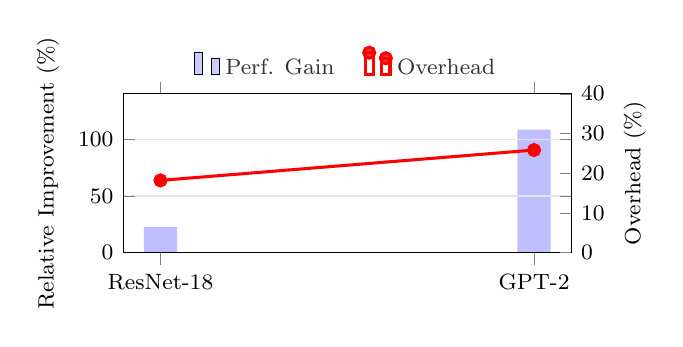
\begin{tikzpicture}
\begin{axis}[
    ybar,
    axis on top,
    width=0.60\linewidth,
    height=3.6cm,
    bar width=12pt,
    ymin=0, ymax=140,
    ylabel={Relative Improvement (\%)},
    symbolic x coords={ResNet-18,GPT-2},
    xtick=data,
    ymajorgrids,
    major grid style={draw=gray!20},
    tick label style={font=\footnotesize},
    label style={font=\footnotesize},
    legend style={
        at={(0.5,1.02)},
        anchor=south,
        draw=none,
        fill=white,
        fill opacity=0.8,
        legend columns=-1,
        /tikz/every even column/.append style={column sep=0.3cm},
        font=\footnotesize
    },
]
\addplot[draw=none, fill=blue!25] coordinates {(ResNet-18,22.6) (GPT-2,108.4)};
\addlegendentry{Perf. Gain}
\addlegendimage{red, mark=*, line width=1.1pt, mark options={fill=red}}
\addlegendentry{Overhead}
\end{axis}

\begin{axis}[
    width=0.60\linewidth,
    height=3.6cm,
    axis x line=none,
    axis y line*=right,
    ymin=0, ymax=40,
    ylabel={Overhead (\%)},
    tick label style={font=\footnotesize},
    label style={font=\footnotesize},
    symbolic x coords={ResNet-18,GPT-2},
    xtick=data,
]
\addplot[red, line width=1.1pt, mark=*, mark options={fill=red}] coordinates {(ResNet-18,18.21) (GPT-2,25.85)};
\end{axis}
\end{tikzpicture}
\vspace{-4pt}
\caption{Cost-Benefit Analysis of set-aware filtering. Bars show relative improvement over pointwise baselines: +22.6\% on CIFAR-10 worst-class accuracy (ResNet-18) and +108.4\% on GPT-2 Distinct-4. The line shows relative overhead from Table~\ref{tab:exp10_time}.}
\label{fig:exp10_overhead}
\vspace{-6pt}
\end{figure}

\paragraph{Exp11 (GPT-2 recursive fine-tuning).} Seeds 1088/2195/4960; streaming PPL runs with checkpoints are under \path{Total_results/Tables/exp11_gpt2_model/Results_streaming/}. We run 5 generations (G0--G4; 10k candidates $\rightarrow$ 2k selected samples per generation). At G4 (mean over 3 seeds): No Filter val PPL $173.30\pm7.66$, Distinct-4 $0.432\pm0.010$; Pointwise val PPL $221.52\pm4.74$, Distinct-4 $0.328\pm0.037$; Set-Aware val PPL $182.22\pm27.96$, Distinct-4 $0.490\pm0.010$. Dispersion (non-learned geometry) and repetition filter baselines are rerun with streaming PPL under \path{Total_results/Tables/exp11_gpt2_model/Results_streaming_ablate/}: Dispersion PPL $196.09\pm13.41$, D4 $0.467\pm0.014$; Repetition Filter PPL $184.44\pm24.10$, D4 $0.488\pm0.029$. MAUVE (G0--G4) is computed with the gpt2-large featurizer at max length 128 using the same Wikitext-103 validation reference; results are in \path{exp11_gpt2_model/MAUVE/dphi1_leash_final_streaming/mauve_g0_g4.csv}. Additional ablations from earlier runs remain under \path{exp11_gpt2_model/Results/}, but the reported numbers in this revision use the streaming PPL protocol.

\paragraph{MAUVE Evaluation Protocol.} Standard Wikitext-103 validation lines exhibit a short-tailed length distribution (about 42\% under 50 words), while GPT-2 generations are much longer. To avoid length-induced shifts in the embedding space from dominating MAUVE, we concatenate the validation split and split it into non-overlapping 128-token chunks using the GPT-2 tokenizer. We then sample 1k chunks as the fixed reference distribution, aligning the reference length with \texttt{max\_text\_length=128} and yielding a stable G0 baseline (MAUVE $\approx 0.203$ in our setup).

\newpage
\section{Additional Experimental Visualizations}
\label{app:viz}
these visuals isolate how the correction mechanism behaves beyond summary tables.

\subsection{Discrete Distribution Collapse (CIFAR-10/GPT-2)}
\begin{figure}[htbp]
\centering
\includegraphics[width=0.95\linewidth]{exp9_11_enhence.png}
{\sloppy\caption{Discrete distribution collapse across CIFAR-10 and GPT-2. Left: the G5 class histogram compares baseline, diversity-only selection (k-Center/DPP), and set-aware filtering; diversity increases spread but does not restore clean pseudo-labels, while set-aware correction recovers minority classes (e.g., classes 3/4). Right: set-aware filtering prevents entropic explosion while maintaining diversity.}\label{fig:exp9_11_enhence}}
\end{figure}

\subsection{Effective Dimension Scan (PCA d-scan)}
\label{app:effective_zone}
\begin{figure}[htbp]
\centering
\includegraphics[width=0.7\linewidth]{Figures/exp11_effective_zone_scan.pdf}
\caption{\textbf{Effective geometric zone scan (GPT-2).} Projection ratio $\|\Pi_d \Delta\ve\|_2/\|\Delta\ve\|_2$ at G0/G4. Mean $\pm$ std over seeds 1088/2195/4960.}
\label{fig:effective_zone_scan}
\end{figure}

\subsection{High-Dimensional Robustness Curve}
\label{app:high_dim_curve}
\begin{figure}[htbp]
\centering
\includegraphics[width=0.95\linewidth]{Figures/exp5_bias_reduction_rate.png}
\caption{High-dimensional robustness. Set-aware dominates up to $d{=}100$; at $d{=}500$ pointwise MLP edges ahead due to sparse geometry.}
\label{fig:exp5_hd}
\end{figure}

\subsection{Adaptive Control Laws}
\label{app:adaptive_control}
\begin{figure}[htbp]
\centering
\includegraphics[width=0.95\linewidth]{exp4_4.2,3_enhence.png}
\caption{Adaptive control under ridge shrinkage and Bayesian prior shift. Left: linear anti-shrinkage control law. Right: suppression-ramp evidence weighting that clamps false-prior regions.}
\label{fig:exp4_adaptive}
\end{figure}

\subsection{Mechanism Analysis: Why Pointwise Baselines Fail in Geometric Drift}
\label{app:viz_mnist}

In Section~\ref{sec:exp_universality}, we demonstrated that pointwise debiasing methods (like DST~\citep{chen2022debiased} and L2AC~\citep{fan2021imbalanced}) fail to correct rotational drift in MNIST. To understand the mechanism, we visualize the learned "correction field" in Figure~\ref{fig:viz_correction_field}.

\begin{figure}[htbp]
\centering
% Please ensure the figure is uploaded with this filename.
\includegraphics[width=0.95\linewidth]{Figures/exp8_mechanism_viz.png} 
\caption{\textbf{Visualization of Learned Correction Fields (MNIST, Generation 50).} 
We compare the correction signals learned by the baseline and our method.
\textbf{Left (DST Bias Head):} The auxiliary bias head in DST operates pointwise. Lacking set-level context, it fails to perceive the coherent rotational drift, predicting a field that resembles random noise or generic blurring. Consequently, the rotation accumulates (MSE $\approx 0.027$).
\textbf{Right (Set-Aware $\Delta\vphi$):} Our Set-Aware filter aggregates information from the candidate set to estimate the global geometric transformation. The learned $\Delta\vphi$ clearly recovers the \textbf{inverse rotation vector field} (tangential flow) required to counteract the $5^\circ$ systematic drift, successfully stabilizing the dynamics (MSE $\approx 0.0003$).}
\label{fig:viz_correction_field}
\end{figure}

\end{document}
